\documentclass[12pt, block=fill]{beamer}
\usepackage{graphicx}
% \usepackage[sfdefault]{FiraSans}
% \usepackage{FiraMono}
% \usepackage[T1]{fontenc}
\usepackage{xcolor}

\usepackage{hyperref}

\definecolor{burntOrange}{rgb}{.8, .5, .1}
\definecolor{textgray}{rgb}{.8,.8,.8}

\newcommand{\alex}[1]{\textcolor{berkeleyYellow}{#1}}
\newcommand{\paul}[1]{\textcolor{red}{#1}}
% \usepackage[normalem]{ulem}

\newcommand{\Z}{\mathbb{Z}}
\newcommand{\R}{\mathbb{R}}
\newcommand{\N}{\mathbb{N}}
\newcommand{\X}{\mathbb{X}}
\newcommand{\indep}{\mathrel{\text{\scalebox{1.07}{$\perp\mkern-10mu\perp$}}}}

\usetheme[
titleformat frame = smallcaps,
subsectionpage = progressbar]
{metropolis}

\metroset{
  block=fill
}

\usepackage{pgfpages}
 \setbeameroption{hide notes} % Only slides
% \setbeameroption{show only notes} % Only notes
% \setbeameroption{show notes on second screen=left} % Both
\setbeamerfont{note page}{size=\footnotesize}


\title{Week 1}
\subtitle{Introduction to Probability}

\author{Paul Laskowski and Alex Hughes}
\institute{UC Berkeley, School of Information}

\begin{document}

\begin{frame}
  \maketitle
\end{frame}

%\begin{frame}
%\footnotesize
%\tableofcontents[hideallsubsections]
%\end{frame}

\section{The Nature of Statistical Models}


\begin{frame}
  \frametitle{What is a Model?}
  \centering
  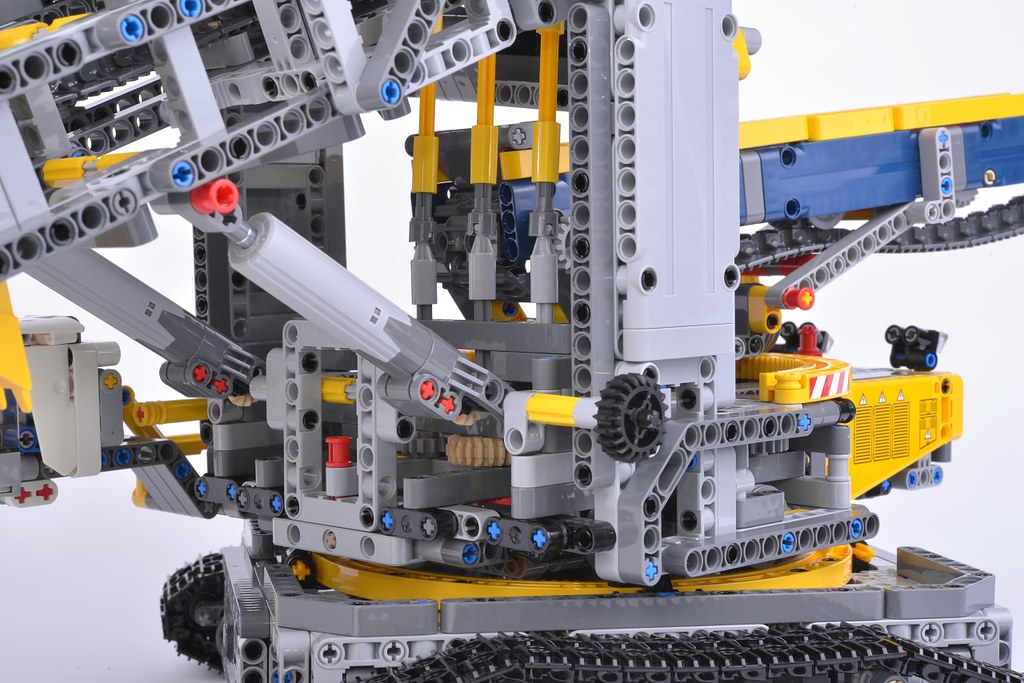
\includegraphics[width=.8\textwidth]{figures/lego_1} \\ 
  \footnotesize Image: www.flickr.com/photos/brickset/ (CC BY
  2.0) 
  \note[item]{This course is about statistical modeling.  So let's
    start by asking, what is a model?} 
  \note[item]{Here's a model, built out of lego bricks.}
  \note[item]{Some of you might have played with legos growing up, I definitely did.}
  \note[item]{The thing with legos is you learn some basic rules: the
    ways that legos can fit together.} 
  \note[item]{Then you can build something that resembles something in
    the real world, that captures important behavior.} 
  \note[item]{When you're starting out with legos for the first time,
    you don't immediately try to build a giant machine.} 
  \note[item]{Maybe you take two legos, test them to see how they fit
    together.  Once you're familiar with the pieces, you can then try
    to create something that you see in the world. } 
\end{frame}

\begin{frame}
  \frametitle{What is a Statistical Model?}
  \centering
  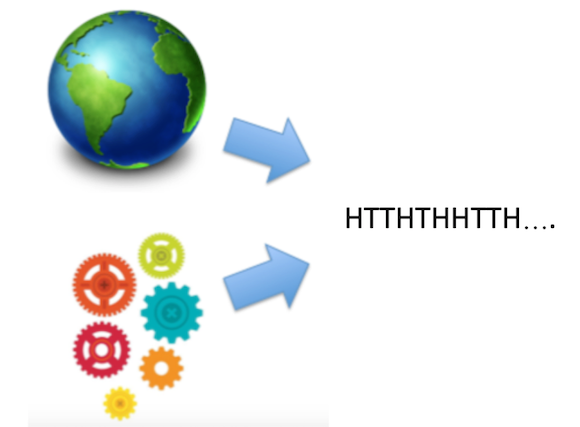
\includegraphics[width=.8\textwidth]{figures/modeling}
  \note[item]{A statistical model is also a representation of something in the world.}
  \note[item]{When you have data, it comes from a real-world system.}
  \note[item]{But we don't just care about this data, we have
    questions: what data is coming next?  what other data could have
    plausible come up? what features of the world are consistent with
    this data?} 
  \note[item]{For those questions, we can't interrogate the world
    directly, we need a statistical model.} 
  \note[item]{This is a representation that also creates data.} 
  \note[item]{We have to pretend that this data actually came from the
    model.  Then we can start to answer these questions.} 
\end{frame}

\begin{frame}
  \frametitle{Course Plan}
  \note[item]{When we designed this course, we decided to follow a
    very strict narrative.} 
  \note[item]{At the highest level of abstraction, here's our plan...}
  \begin{enumerate}
\item Putting together statistical models
\item Fitting models to data
\end{enumerate}

\note[item]{Most courses jump around, looking at data, then building models, then back.}
\note[item]{We believe it's better to really commit to understanding models, then apply them.}
\note[item]{Because of that, we're actually not going to touch any data for several weeks.}
\note[item]{But don't worry, there will be a LOT of application in the second half of the course.}

\end{frame}


\begin{frame}
  \frametitle{First Models}
  \note[item]{When we start out, our models are not going to resemble the world at all}
  \note[item]{They will be brittle - with no flexibility to make them look like the real world}
  \note[item]{Actually, just like this tower of legos, they may be very rectangle.}
  \note[item]{You may ask, where did this rectangular distribution come from?}
  \note[item]{The answer is we made it up!  and we just want to build
    something simple to understand how the bricks fit together}
  \centering 
  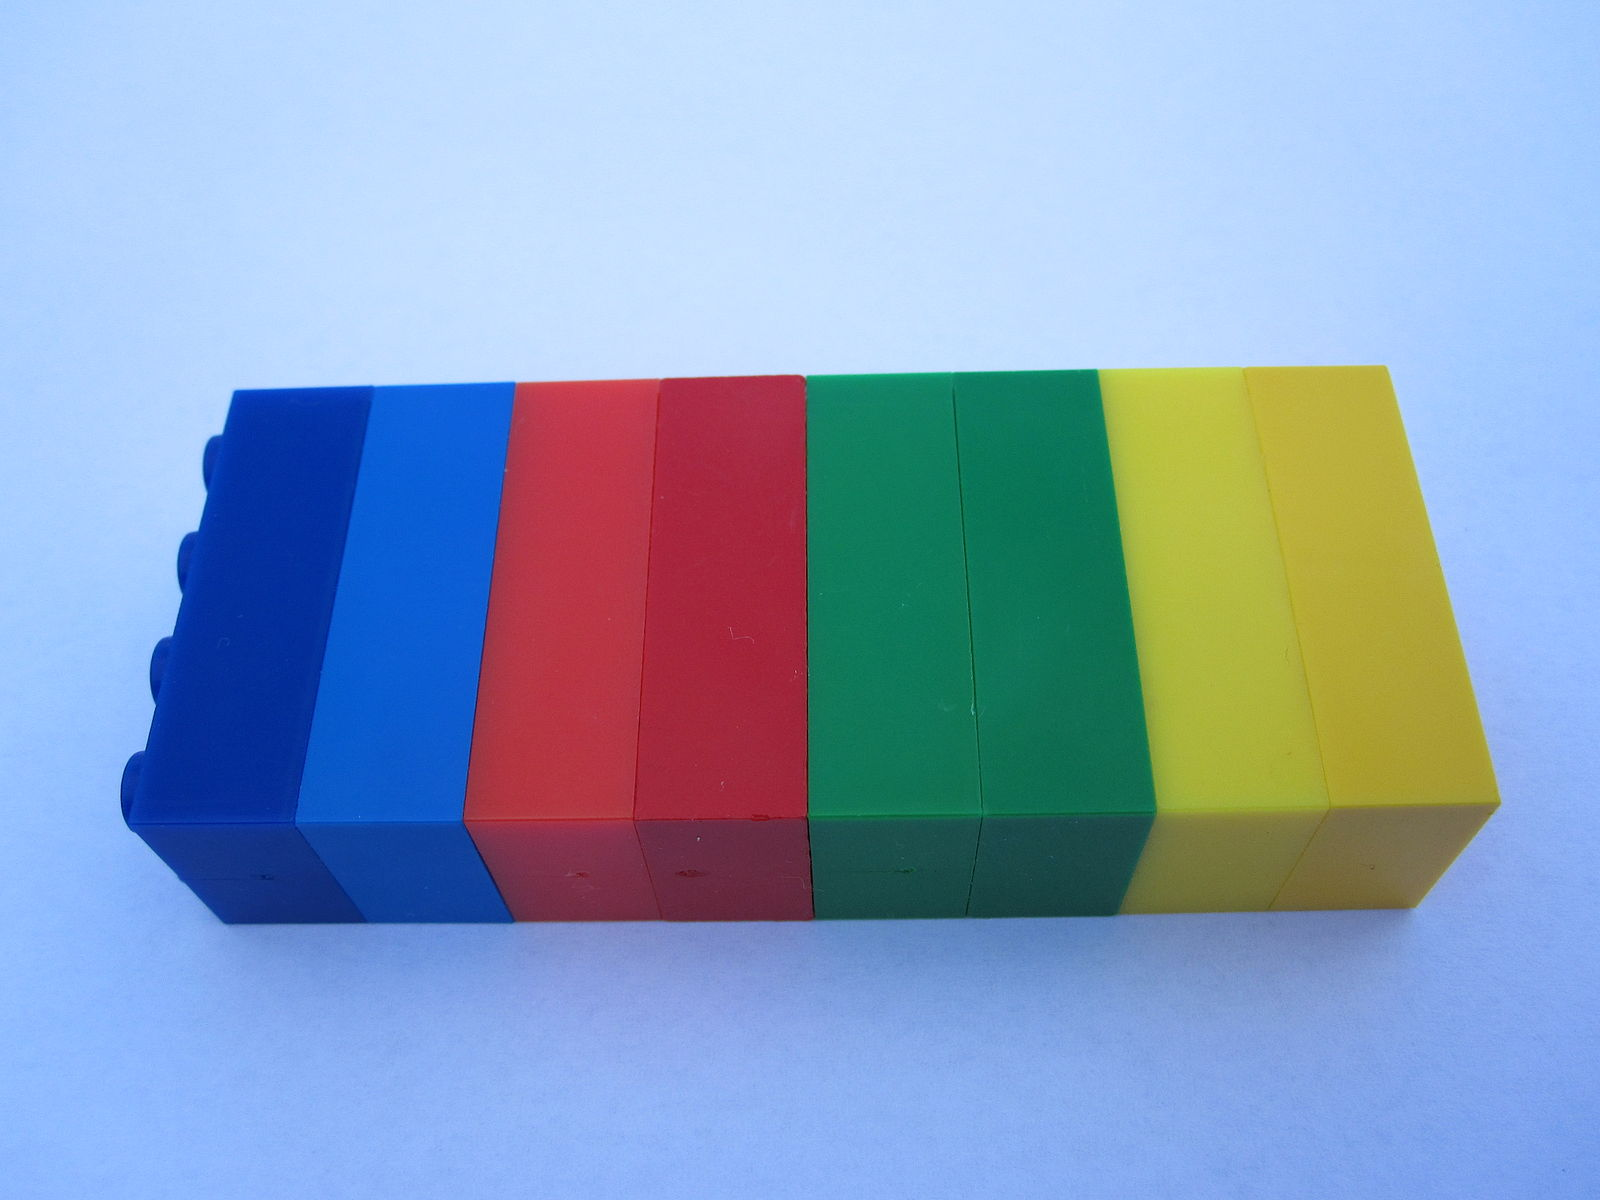
\includegraphics[width=.8\textwidth]{figures/legos_3} \\ 
  \footnotesize Image: Hans Schou (CC BY-SA 3.0)
\end{frame}

\begin{frame}
  \frametitle{Useful Models}
  \centering 
  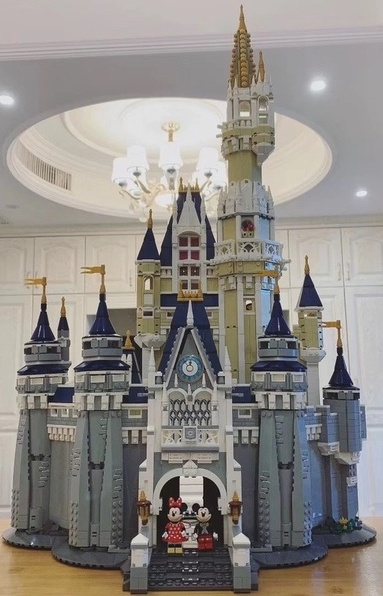
\includegraphics[width=.4\textwidth]{figures/disney_castle} \\ 
  \footnotesize Image: www.flickr.com/photos/brickset/ (CC BY 2.0)
  \note[item]{But the key is not to worry about those problems at the
    beginning.  as we learn more, we'll see that our models can be
    more flexible, to represent a wide range of real world systems} 
  \note[item]{We'll also learn how to fit our models to data, and
    that's going to make them really useful.} 
\end{frame}


\begin{frame}
  \frametitle{Probability is Rules for Putting Pieces Together}

  \centering 
  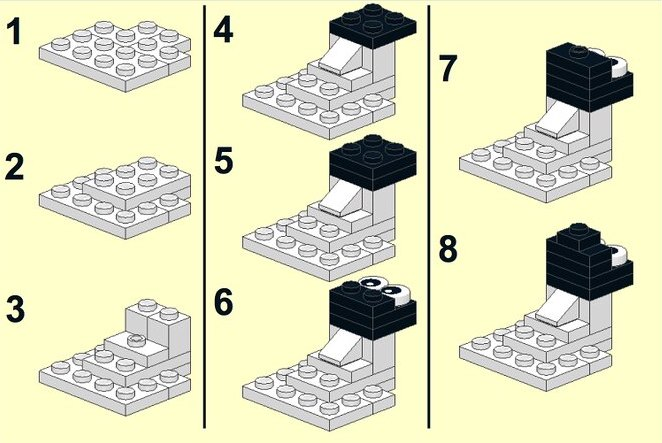
\includegraphics[width=.8\textwidth]{figures/sheep} \\ 
  \footnotesize Image: www.flickr.com/photos/billward/ (CC BY 2.0)
  \note[item]{This week, we're starting with the foundation.  probability theory}
  \note[item]{This is really the nuts and bolts, how do the pieces of
    statistical models fit together.} 
  \note[item]{A strong understanding of probability will be useful to
    you through this course and through your career as a data
    scientist.} 
\end{frame}

\section{Unit Plan}

\begin{frame}
  \frametitle{Necessary Foundation}
  
  \begin{itemize}
  \item  A precise definition of probability
  \item  How mathematicians build from a set of axioms to useful properties
  \item How to connect these properties to problems that we want to solve
 \end{itemize}
  
\end{frame}

%\begin{frame}
%  \frametitle{Lack of Evidence}
%  \begin{align*} 
%    P(S | C_{m}, O_{w}, X) &> P(S | C_{m}, O_{m}, X) \\ \\ 
%    \frac{P(C_m | S, O_w, X) \times P(S | O_w, X)}{P(C_m | O_w, X)} &
%  \vspace {1em}
%  > \frac{P(C_m | S, O_m, X) \times P(S | O_m, X)}{P(C_m | O_m, X)}
%  \end{align*} 
%\end{frame}


%Section 1.4 Edits start here
% We're keeping this content in as a comment, but it was initially recorded by
% Coye, and we have removed this part of the lecture from the course.

% \section{Statistical Models}

% \begin{frame}
%   \frametitle{Quote by Chris Anderson, \textit{Wired} Magazine}
%   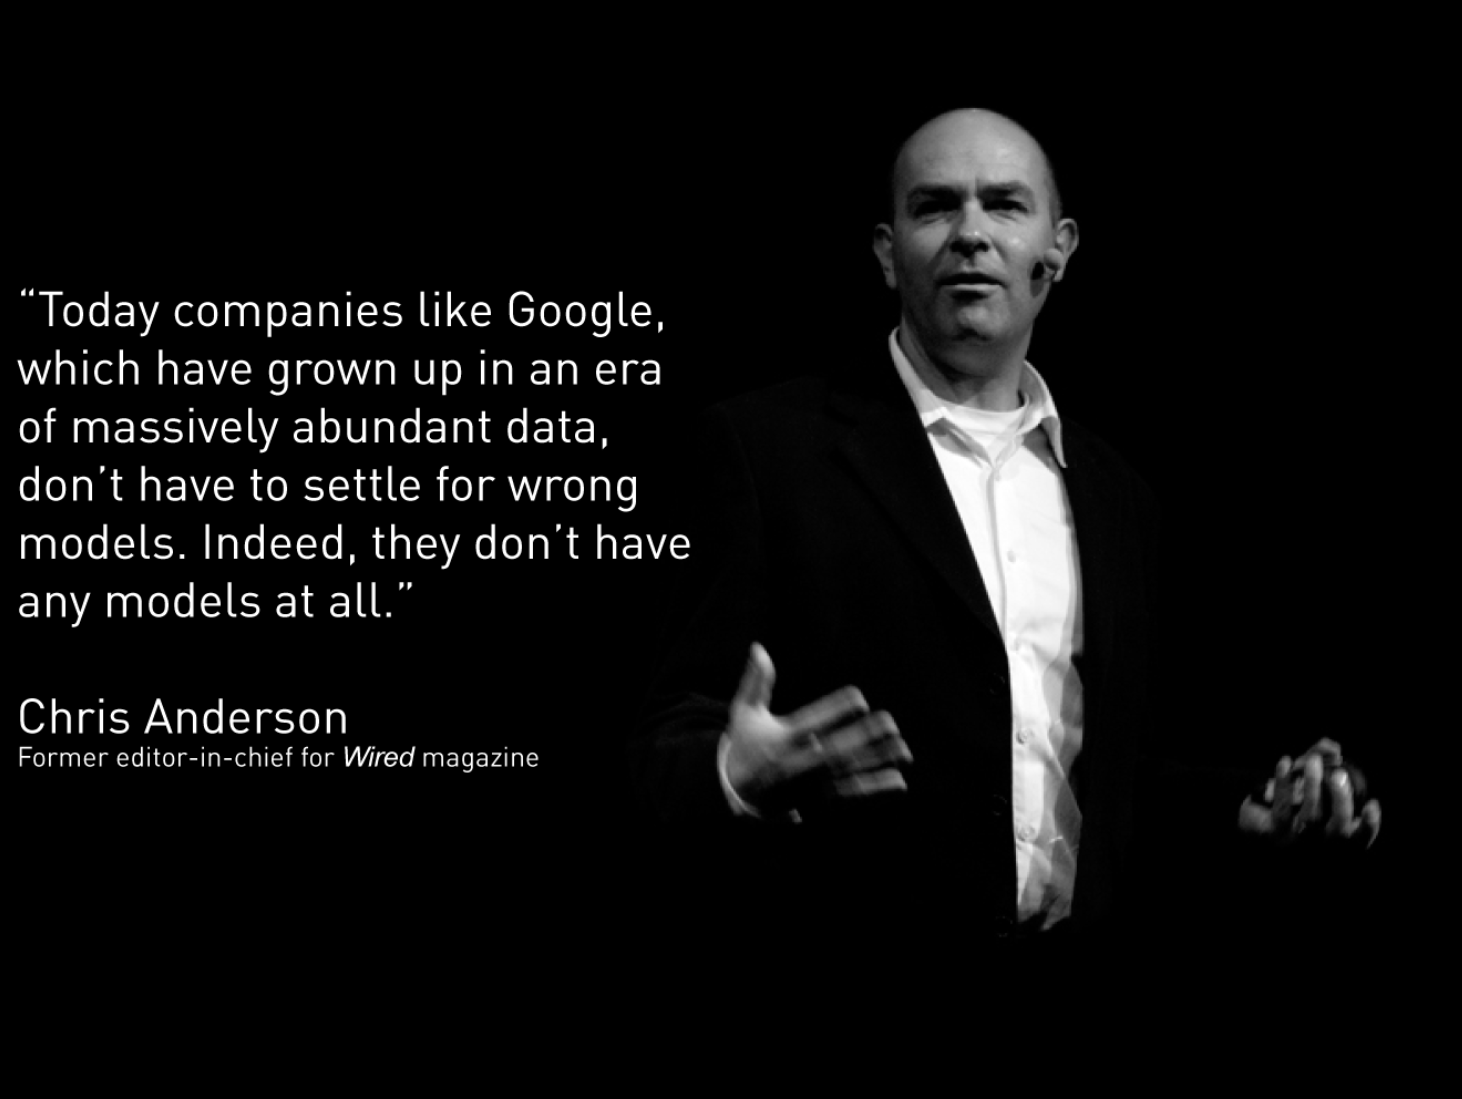
\includegraphics[width=1.0\linewidth]{figures/chris_anderson_quote.png}
% \end{frame}

% \begin{frame}
%   \frametitle{What is a model?}
%   \begin{center}
%     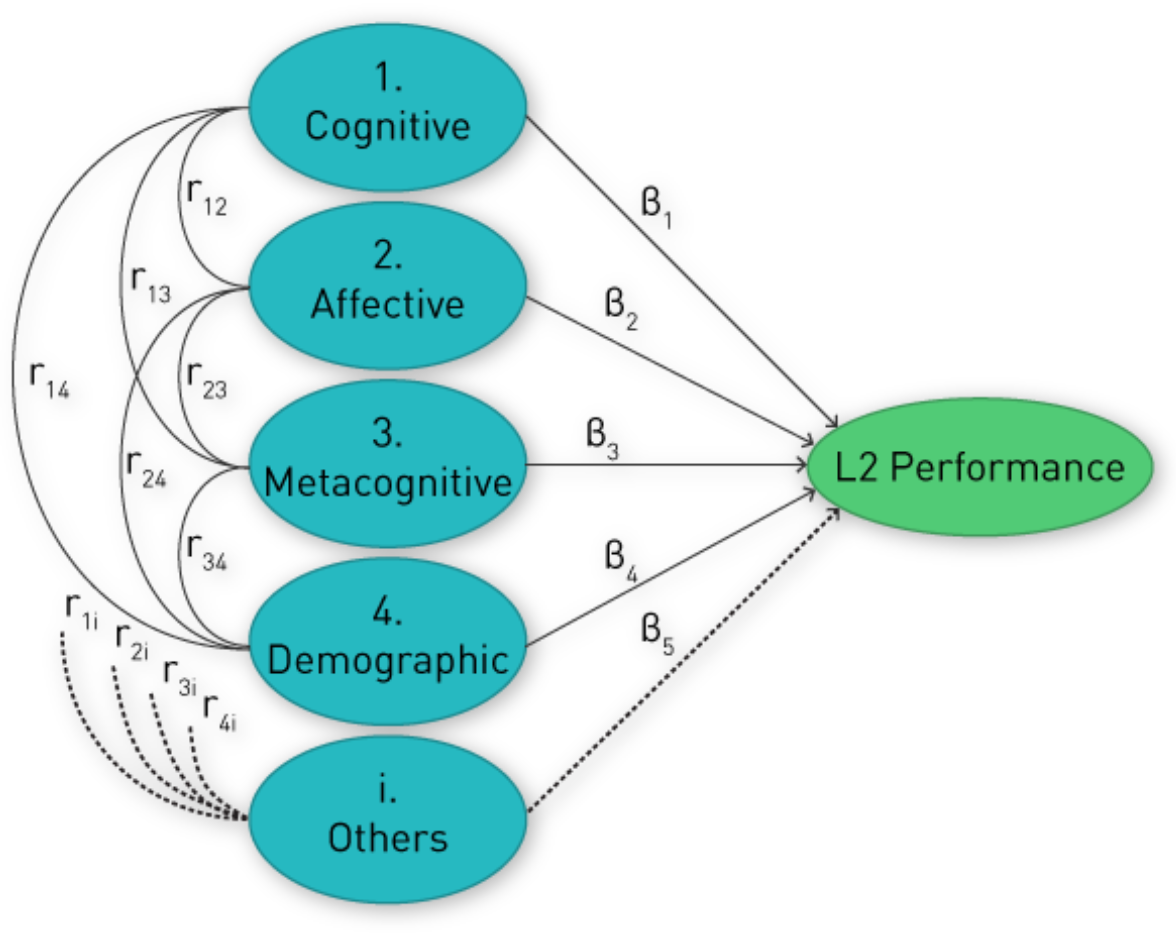
\includegraphics[width=0.5\linewidth]{figures/model_a.png}
%     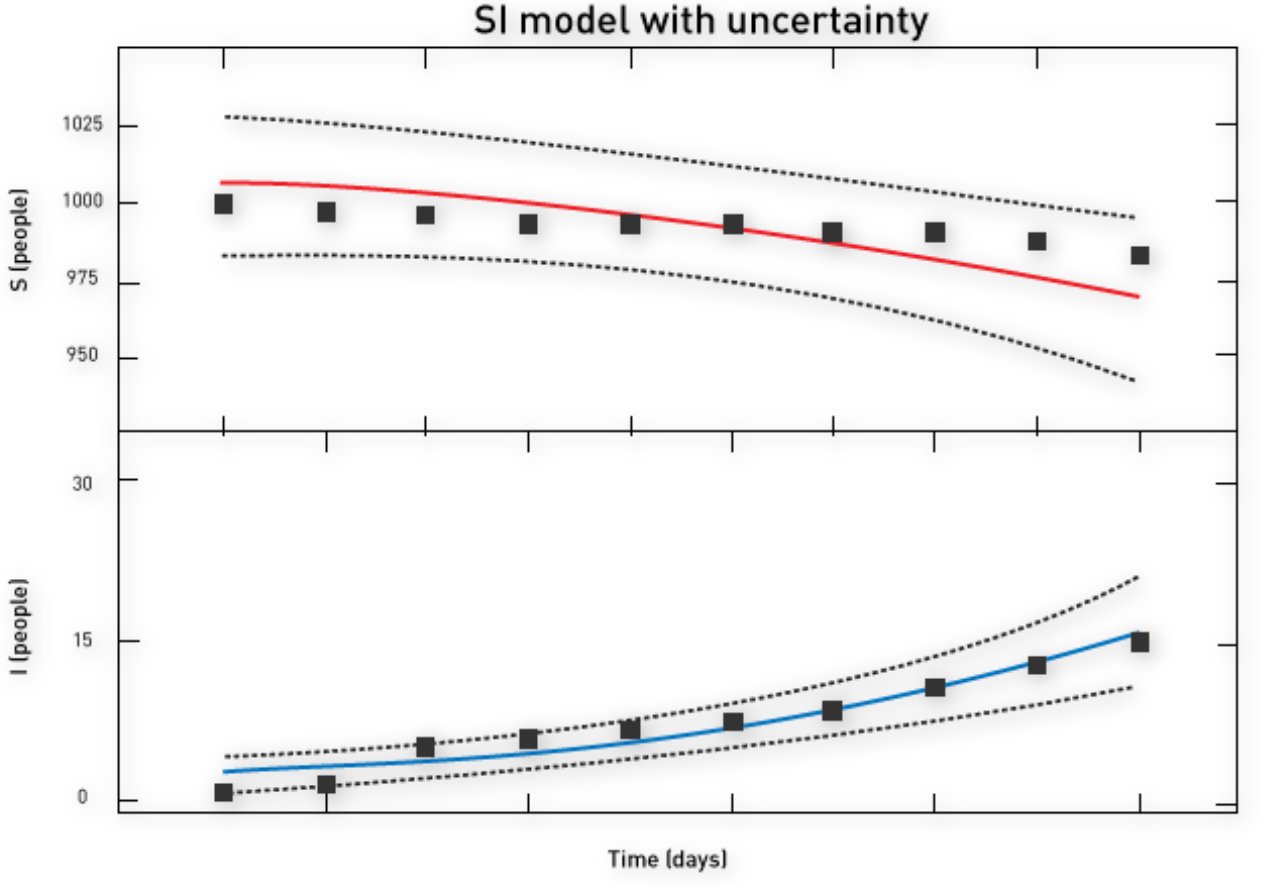
\includegraphics[width=0.5\linewidth]{figures/model_b.png}
%   \end{center}
% \end{frame}

% \begin{frame}
%   \frametitle{What is a model?}
%   \begin{center}
%     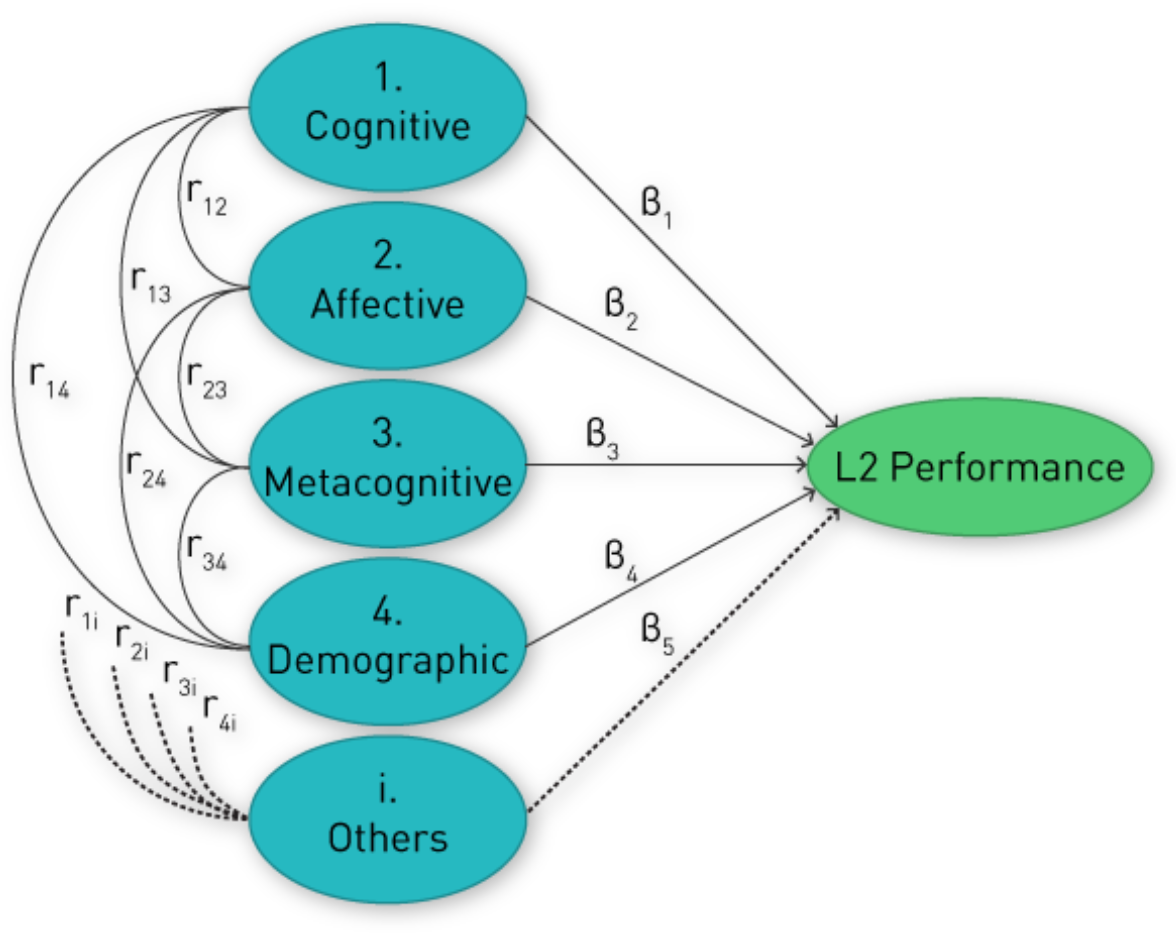
\includegraphics[width=0.9\linewidth]{figures/model_a.png}
%   \end{center}
% \end{frame}

% \begin{frame}
%   \frametitle{What is a model?}
%   \begin{center}
%     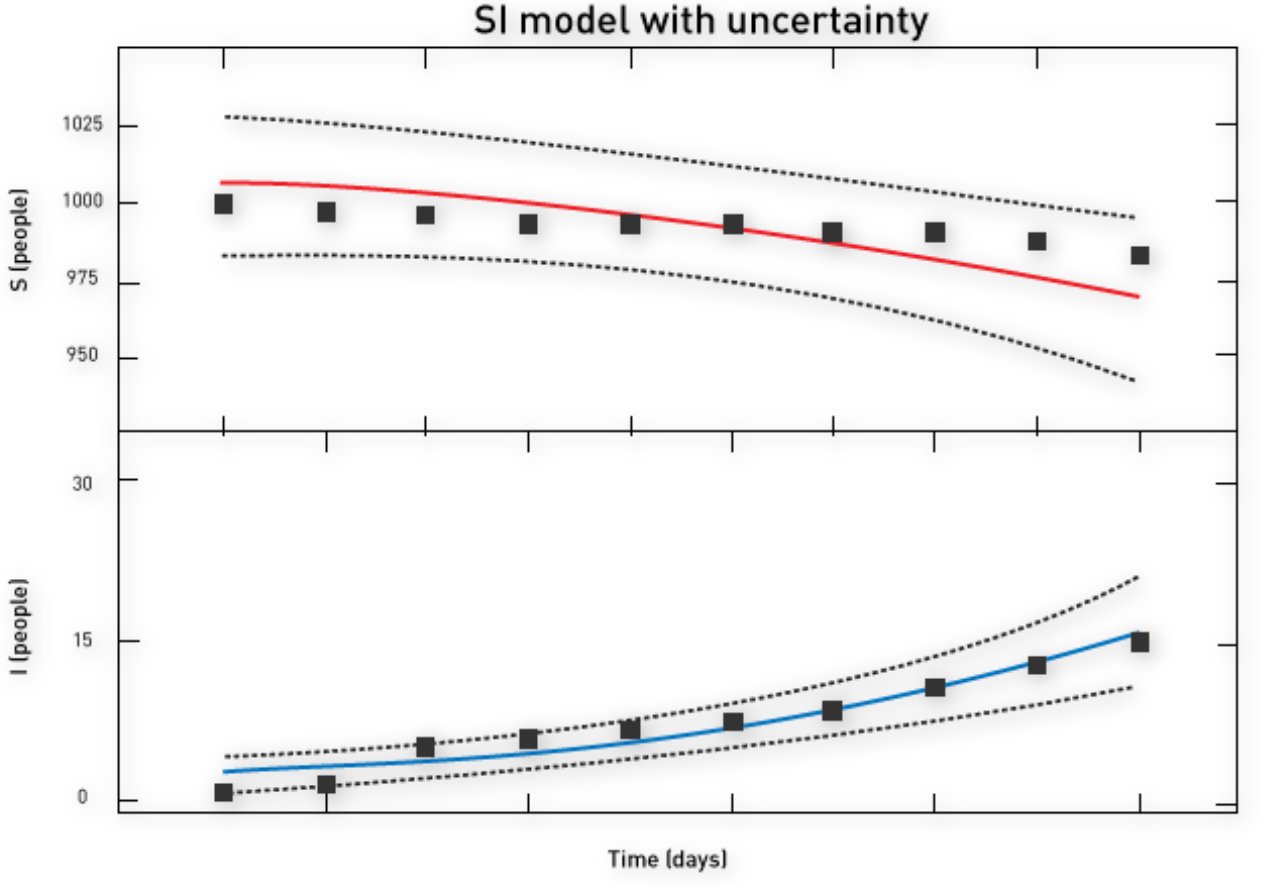
\includegraphics[width=0.9\linewidth]{figures/model_b.png}
%   \end{center}
% \end{frame}

% \begin{frame}
%   \frametitle{A Simple Model}
%   \begin{center}
%     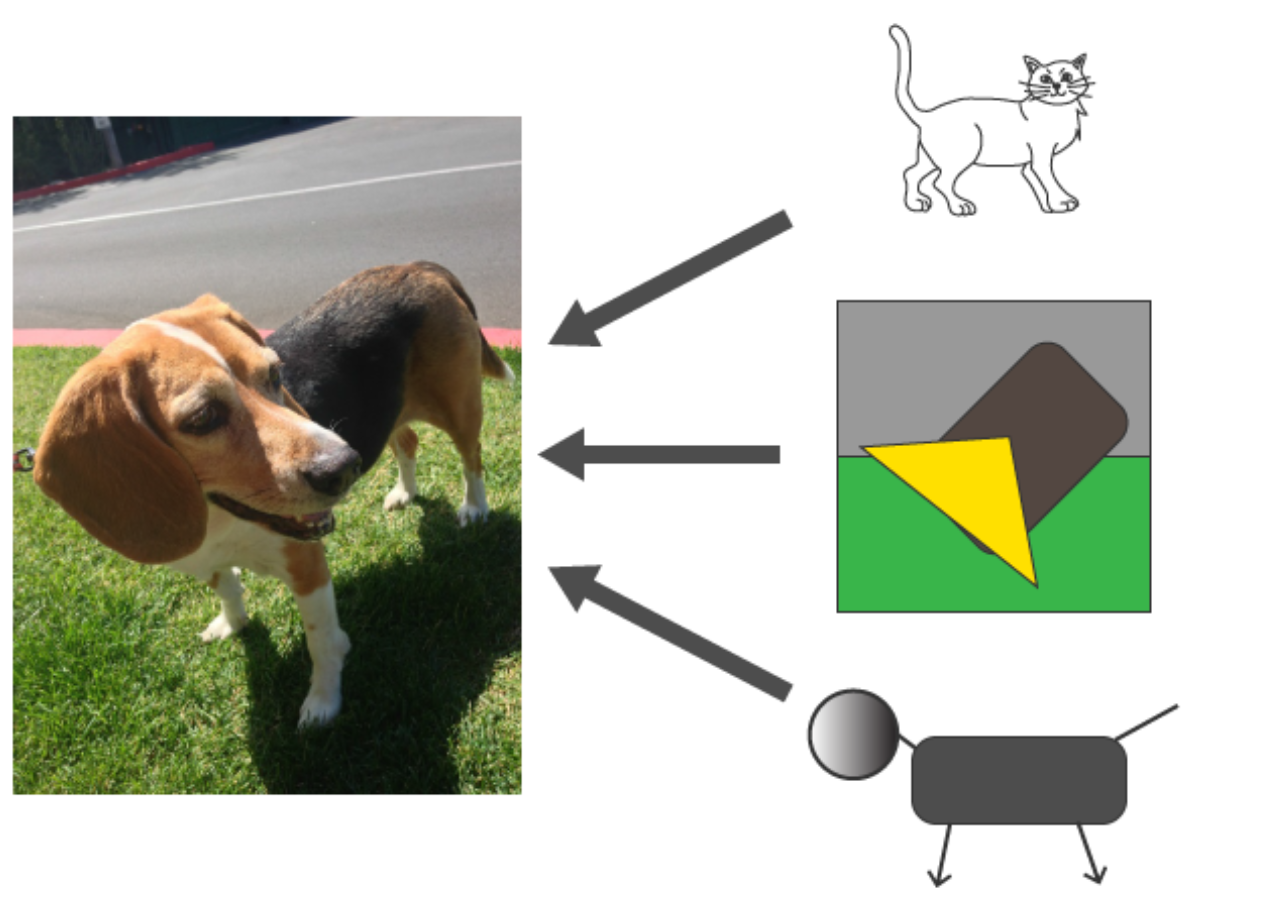
\includegraphics[width=0.9\linewidth]{figures/model_c.png}
%   \end{center}
% \end{frame}

% \begin{frame}
%   \frametitle{A Simple Model}
%   \begin{center}
%     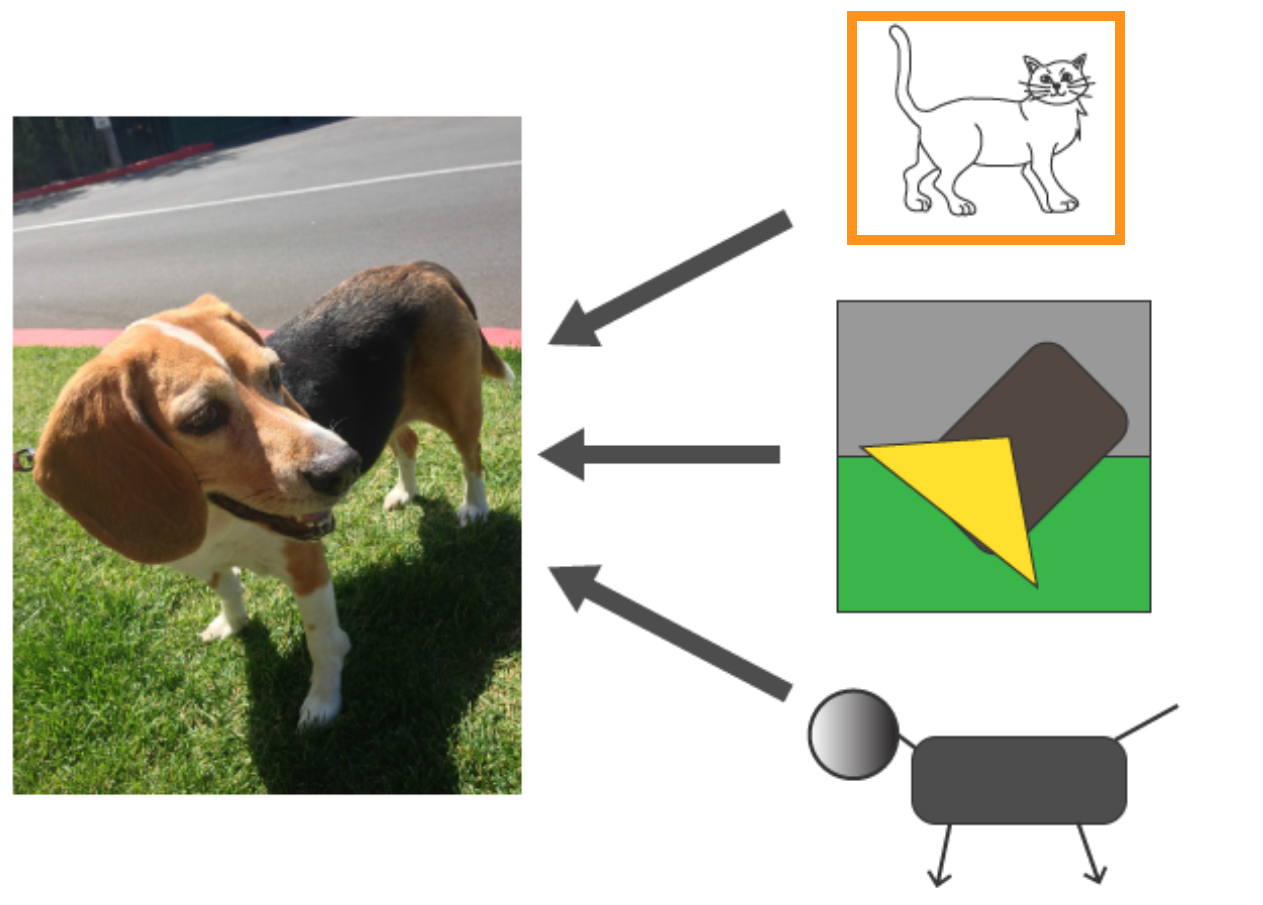
\includegraphics[width=0.9\linewidth]{figures/model_c1.png}
%   \end{center}
% \end{frame}

% \begin{frame}
%   \frametitle{A Simple Model}
%   \begin{center}
%     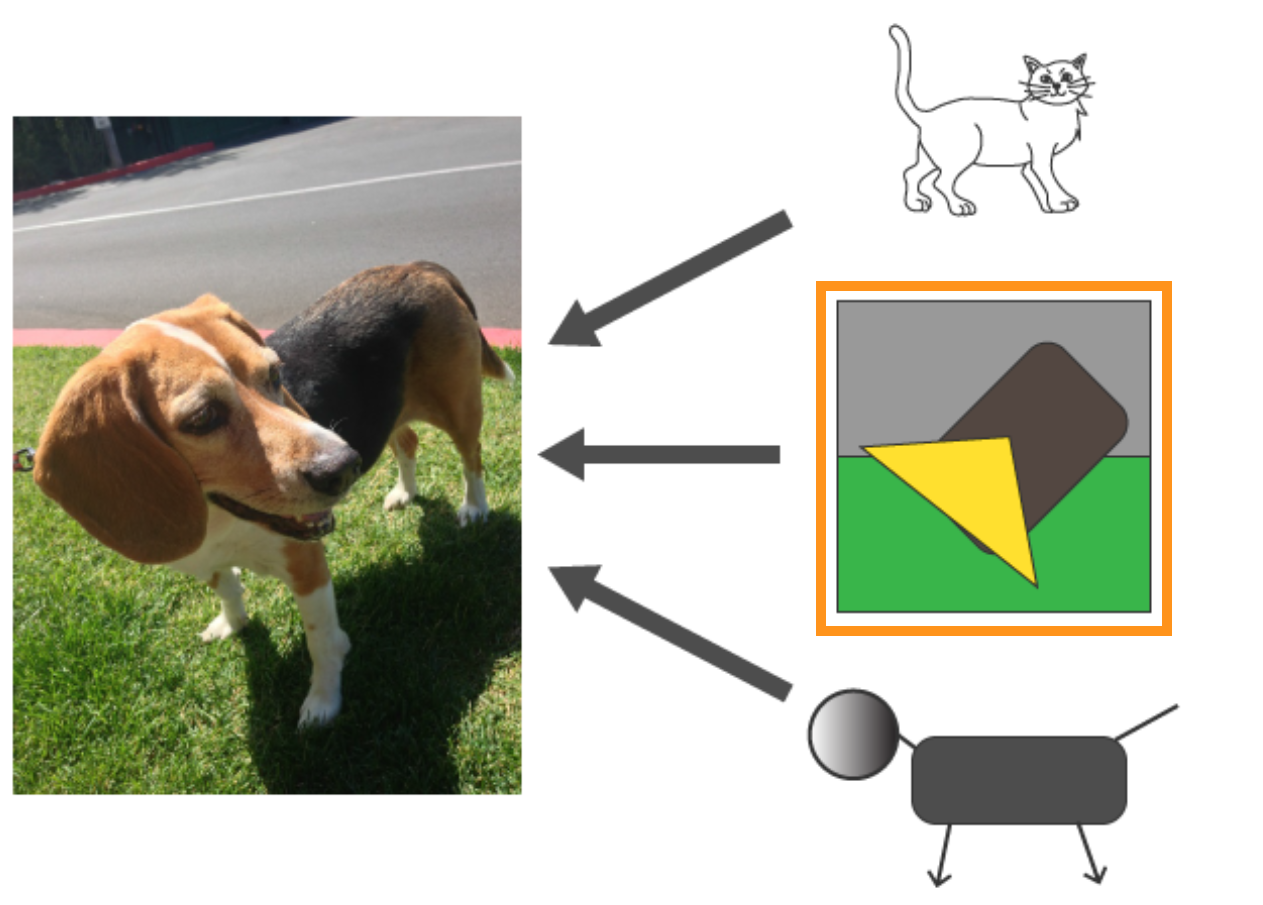
\includegraphics[width=0.9\linewidth]{figures/model_c2.png}
%   \end{center}
% \end{frame}

% \begin{frame}
%   \frametitle{A Simple Model}
%   \begin{center}
%     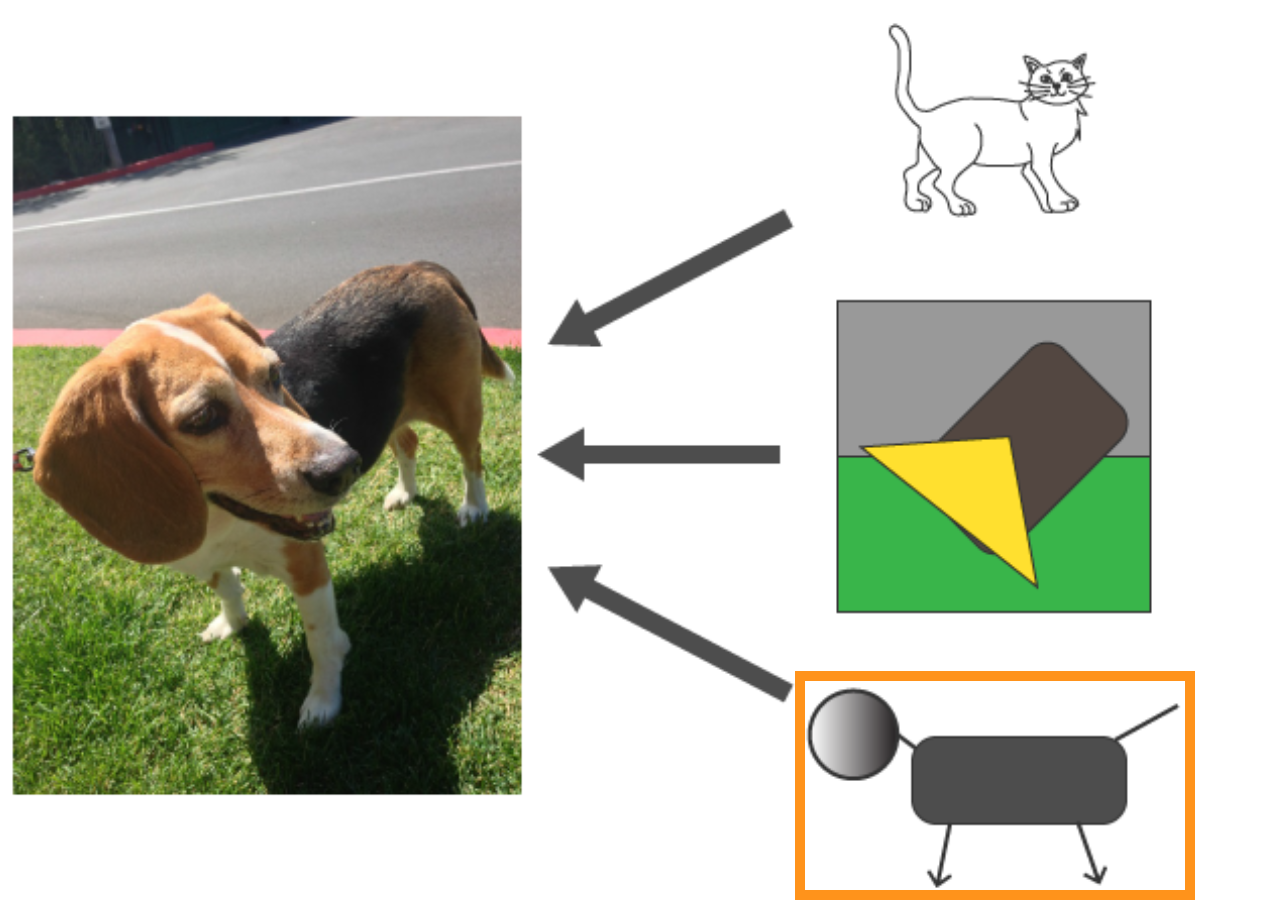
\includegraphics[width=0.9\linewidth]{figures/model_c3.png}
%   \end{center}
% \end{frame}

% \begin{frame}
%   \frametitle{A Simple Model}
%   \begin{columns}
%     \column{0.4\textwidth}
%       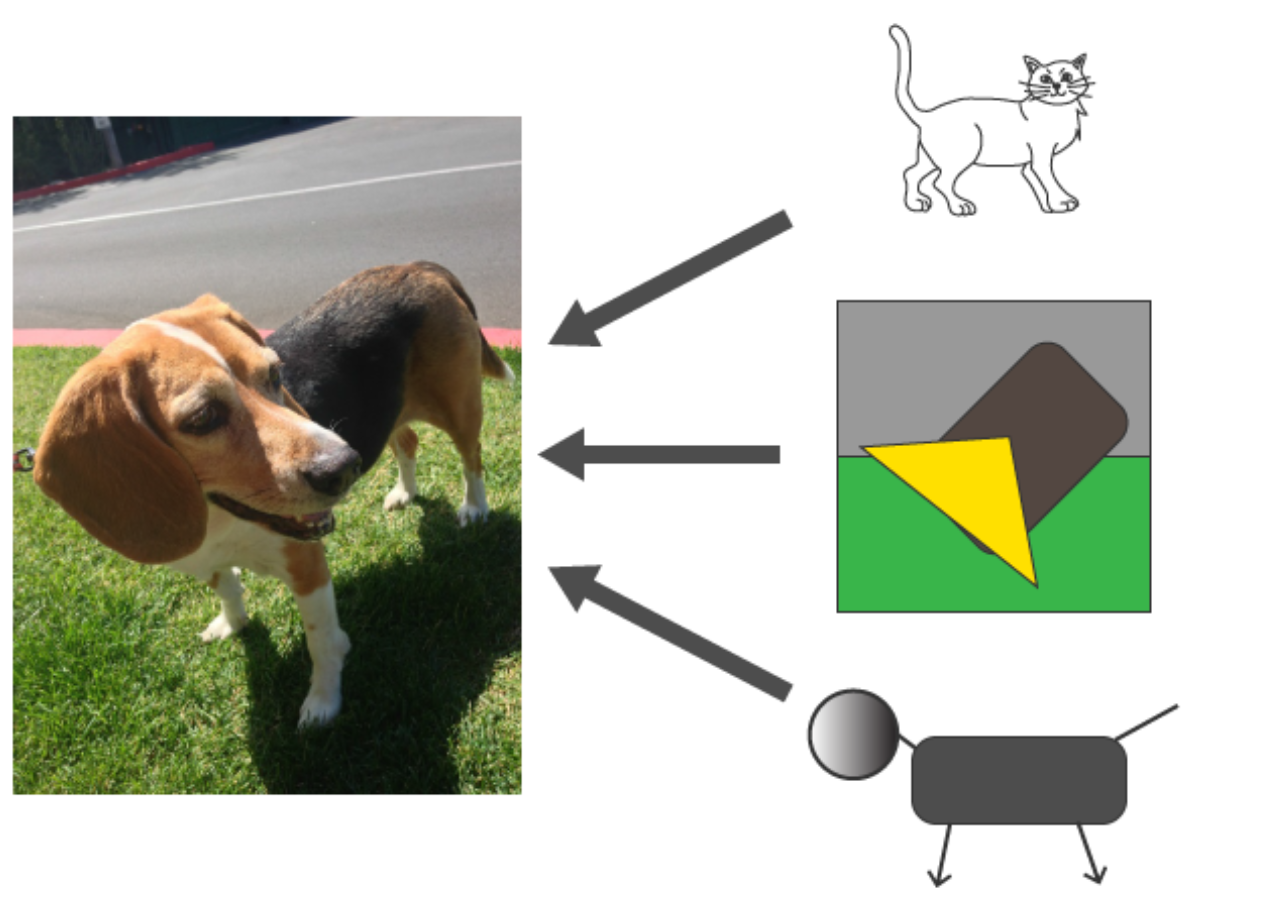
\includegraphics[width=1.0\linewidth]{figures/model_c.png}

%     \column{0.6\textwidth}
%       \begin{itemize}
%       \item None of these models are perfect
%       \item They are all representations, capturing some aspects of this thing that exists in the real world
%       \item That is what a model does!
%       \item We create these so that we can examine them and see if we can get a pretty good estimate of something that exists in the real world
%   \end{itemize}
%   \end{columns}

% \end{frame}

% \begin{frame}
%   \frametitle{Quote by George Box, Statistician}
%   \begin{center}
%     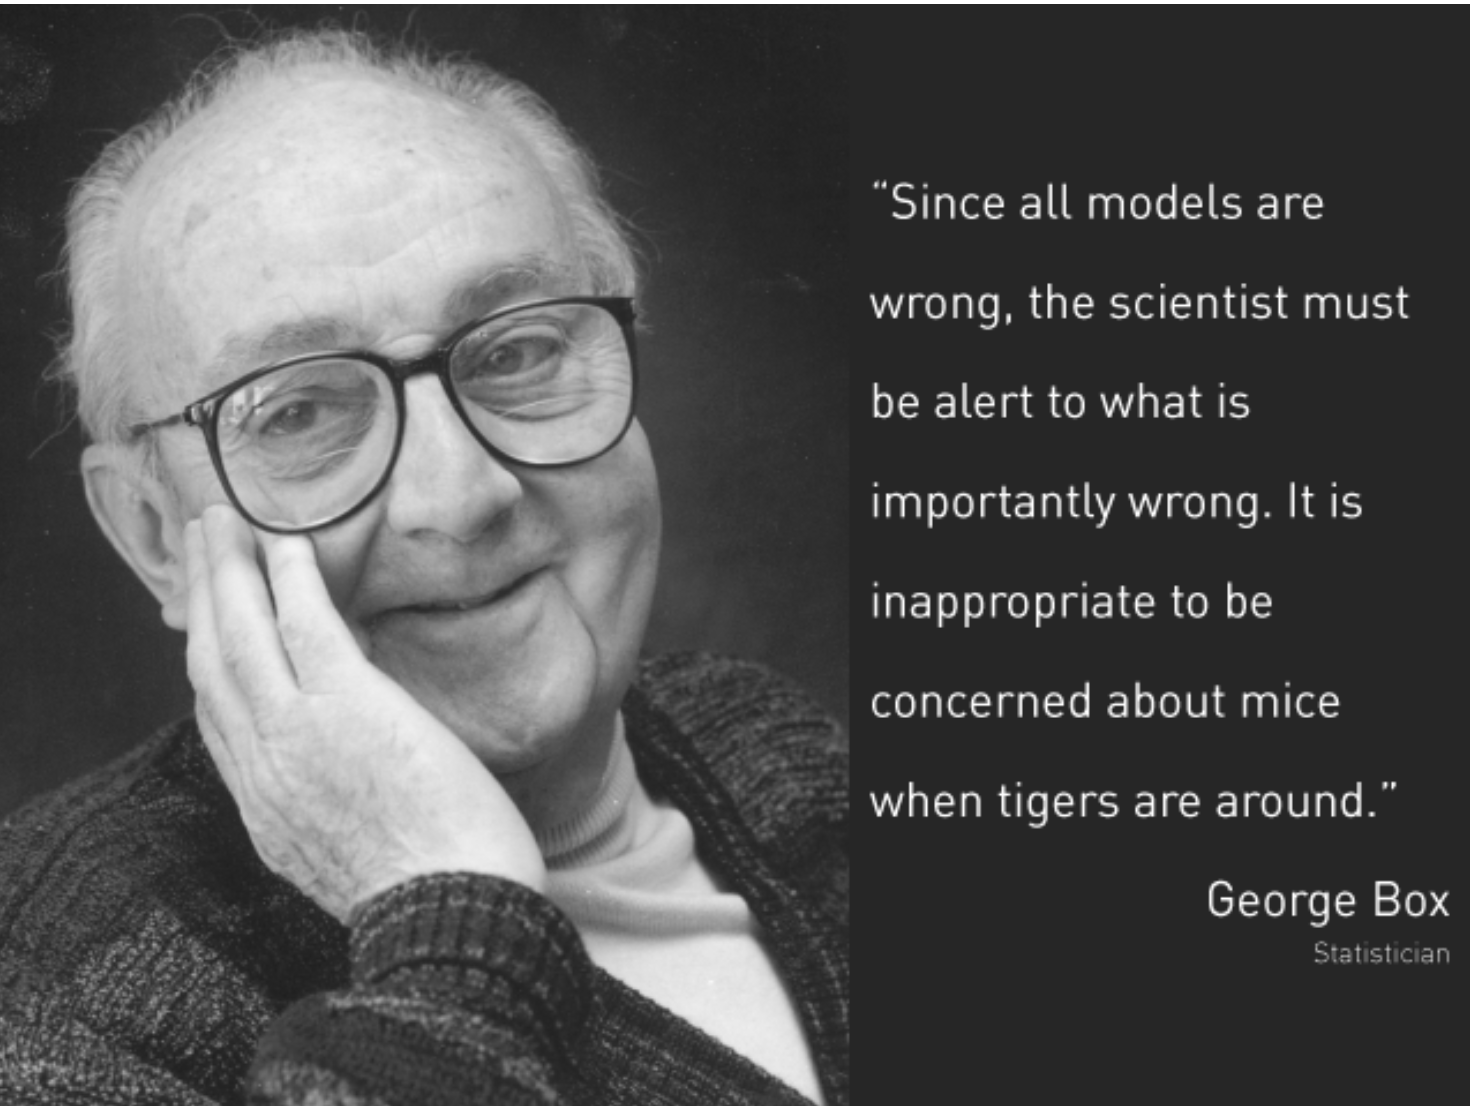
\includegraphics[width=0.9\linewidth]{figures/george_box_quote_a.png}
%   \end{center}
% \end{frame}

% \begin{frame}
%   \frametitle{Successful Models}
%   \begin{enumerate}
%       \item Present logical relationships between data
%       \item Avoid preoccupation with small details
%       \item Convey information simply and clearly
%   \end{enumerate}
% \end{frame}

% \begin{frame}
%   \frametitle{Quote by George Box, Statistician}
%   \begin{center}
%     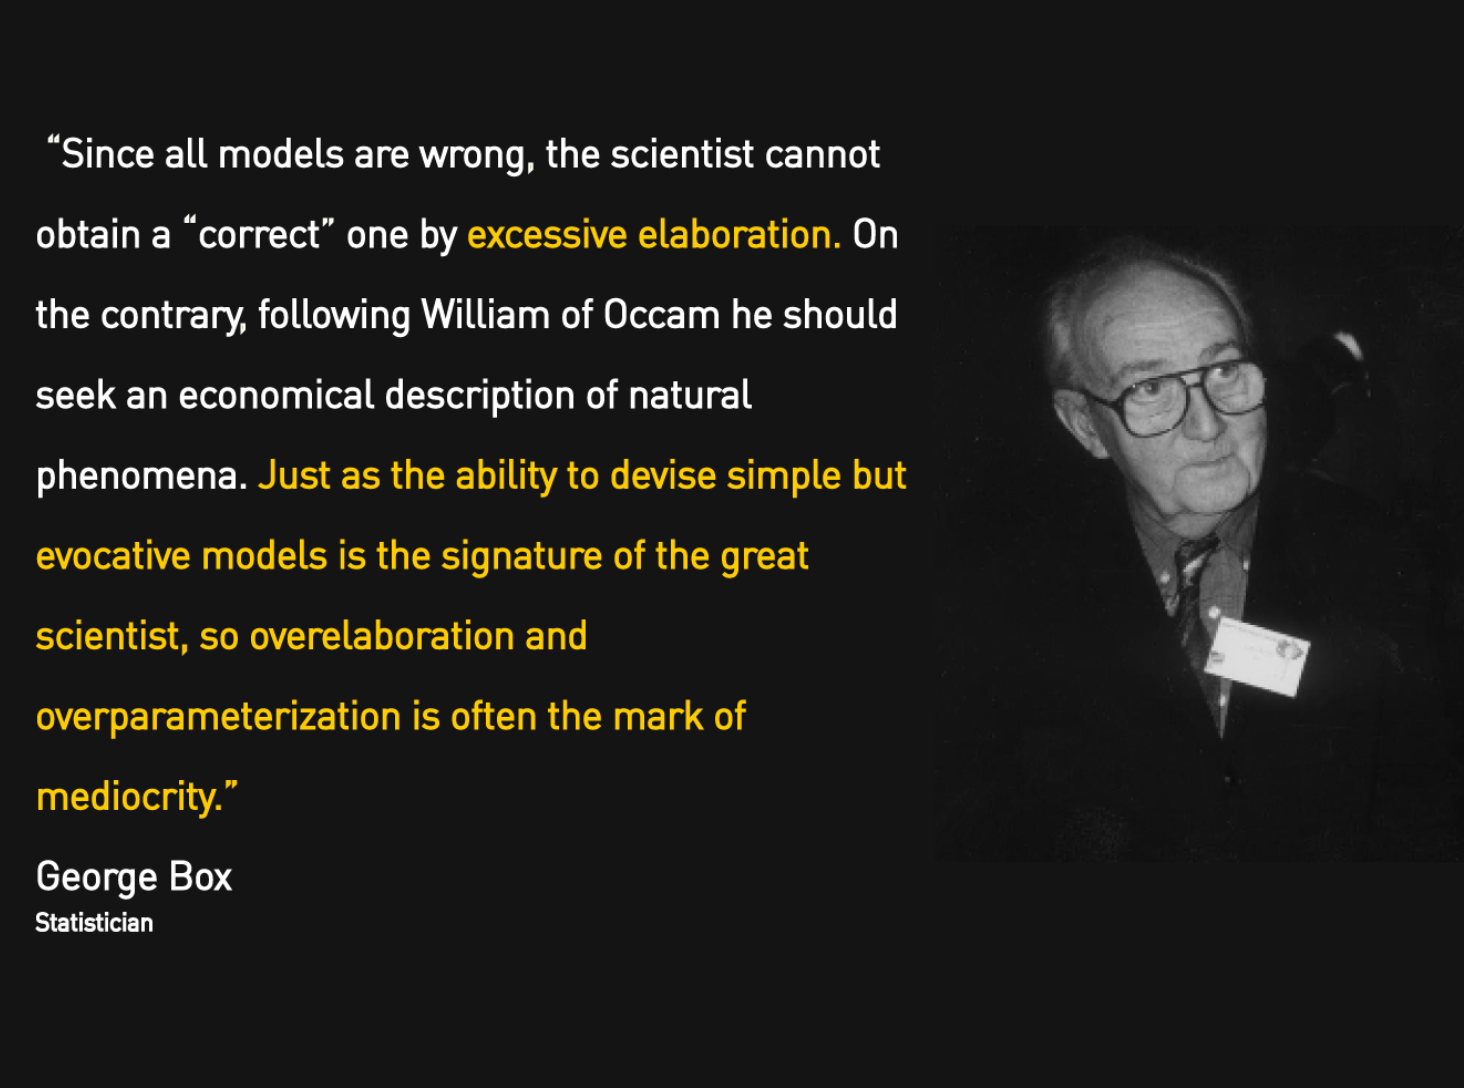
\includegraphics[width=0.9\linewidth]{figures/george_box_quote_b.png}
%   \end{center}
% \end{frame}


% \begin{frame}{Frame Title}
%   \frametitle{Simplicity vs. Complexity}

% \begin{itemize}
%     \item Emphasizes pieces of key information simply
%     \item Allows clear understanding of what is going on within the data
%     \item Answers \textbf{"why"}
% \end{itemize}
% \end{frame}

%
% Section 1.4 Edits End here


\section{Reading Assignment}

\begin{frame}
  \frametitle{Reading Assignment}
  Throughout this course, we intersperse reading, lectures, and work
  that you complete as a bundled \textit{async}. This way, you can
  very quickly move from 
  \begin{itemize}
  \item An introduction to a concept
  \item An explanation of its use
  \item A proof of that concept 
  \item An application using data or problem solving
  \end{itemize}
  We have designed the course so that you can complete the async,
  reading, and lecture activity components over a few self-contained
  study sessions.
\end{frame}

\begin{frame}
  \frametitle{Reading Assignment (cont.)}
  Read the following sections:

  \begin{itemize}
  \item Introduction, page xv - xviii
  \end{itemize}
  \note[item]{What do we actually say in this?}
\end{frame}

\section{Probability is Reasoning Under Uncertainty}

\begin{frame}
  \frametitle{Probablity is A System of Reasoning}

  \begin{columns}
    \begin{column}{0.6\textwidth}
      "Essentially, the theory of probability is nothing but good common
      sense reduced to mathematics. It provides an exact appreciation of
      what sound minds feel with a kind of instinct, frequently without
      being able to account for it.”\\ 
      - Pierre-Simon Laplace
    \end{column}
    \begin{column}{0.4\textwidth}  
      \begin{center}
        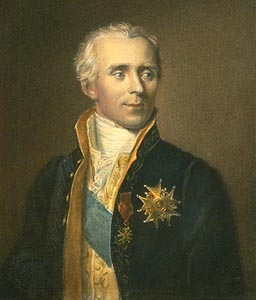
\includegraphics[width=\textwidth]{figures/Laplace}
      \end{center}
    \end{column}
  \end{columns}
  
  \note[item]{How would you define probability?  Is it something
    that you encounter in your day-to-day life?  A measure of
    randomness in the world?} 
  \note[item]{Laplace was a famous mathematician, who developed what
    we call the Bayesian interpretation of probability.  Let's read
    what he said in 1814.} 
  \note[item]{Laplace believed that, as humans, we are natural
    processors of probability.  We think in probabilities, we use
    probability when we speak to each other.}   
  \note[item]{So of course we think of probability as existing out in
    the natural world.} 
  \note[item]{But, I'm here to tell you that probability is actually a
    model.} 
  \note[item]{That's right, the randomness that we perceive around us
    is a model that we use to make sense of the world. } 
  \note[item]{Let me try to convince you with a few examples.} 

  % Others to consider:
  % 
  % “For every action, there's an infinity of outcomes. Countless trillions are possible, many milliards are likely, millions might be considered probable, several occur as possibilities to us as observers - and one comes true.”
  % ― China Miéville, The Scar
  % 
  % “A likely impossibility is always preferable to an unconvincing possibility. The story should never be made up of improbable incidents; there should be nothing of the sort in it.”
  % ― Aristotle, Poetics
\end{frame}


\begin{frame}
  \frametitle{Probability is A Model of the World}
  \begin{block}{Apocryphal quotations}
    ``\textit{All models are wrong; some are useful.}'' \\
    \hspace{1em} —George Box
  \end{block}

  Probability is:

  \begin{itemize}
  \item A mathematical construct
  \item A model or abstraction of the world 
%  \pause
%    \begin{itemize}
%    \item Events are not random, with full information
%    \item Full information is impossible
%    \end{itemize}
  \end{itemize}

  \note[item]{But I'm here to tell you that probability is just a
    model.  It's a very useful model - one that we can make
    mathematically precise.  But it's a model of the world.} 
  \note[item]{Let me try to convince you with a few examples.} 
  \note[item]{\paul{Not sure how to fit the box quote into the
      narrative - wonder if there's something more specific to
      probability.}} 
\end{frame}

\begin{frame}
  \frametitle{Probability is a Model - Example 1}
  \centering 
  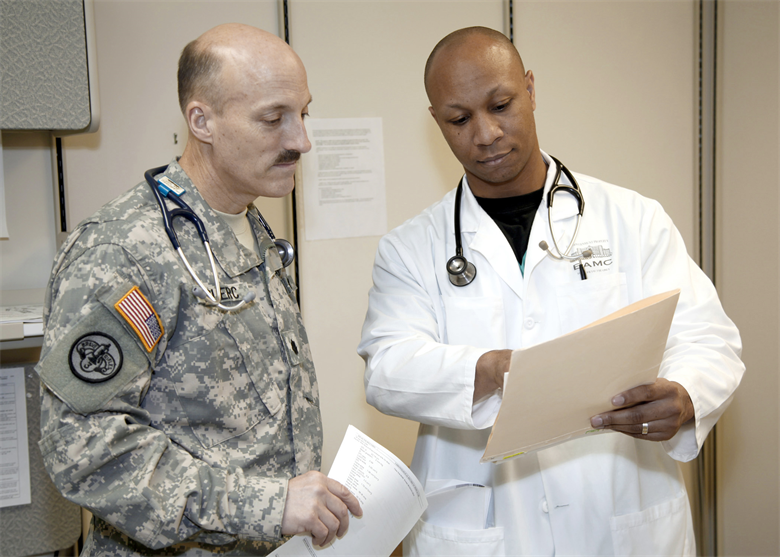
\includegraphics[width=0.8\textwidth]{figures/mil_doctors}
  \note[item]{First, say that you go to the doctor with some abdominal
    pain.} 
  \note[item]{The doctor tells you that you have a 80\% chance of
    having kidney stones.} 
  \note[item]{But is there any randomness in whether you have kidney
    stones?} 
  \note[item]{If you walk out of the office and come back the next
    day, will you have kidney stones 80\% of the time?} 
  \note[item]{Of course not.  There's no randomness, you either have
    kidney stones or you don't.} 
  \note[item]{The doctor is using probability in what we call it's
    subjective sense -- as a strength of belief.} 
\end{frame}

\begin{frame}
  \frametitle{Probability is a Model - Example 2}
  \centering 
    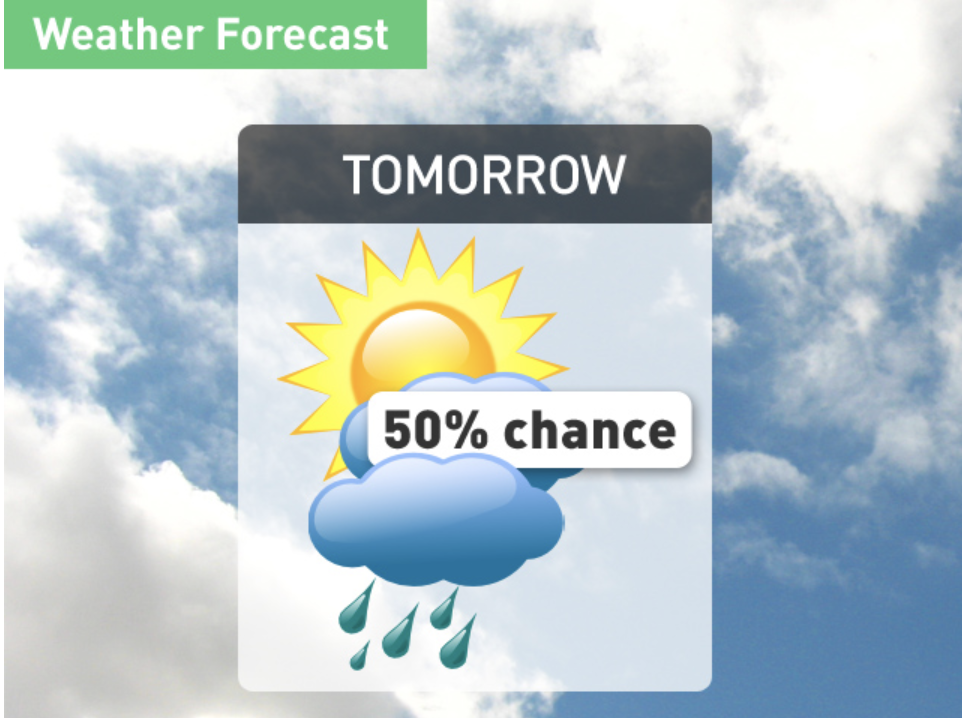
\includegraphics[width=.8\textwidth]{figures/forecast}
  \note[item]{Next, you look at the weather forecast and you see that
    there's a 50\% chance of rain tomorrow.} 
  \note[item]{Is there any randomness in whether it will rain?  It's a
    future event, so you might think maybe.} 
\end{frame}

\begin{frame}
  \frametitle{Probability is a Model - Example 2 (cont.)}
  \centering 
    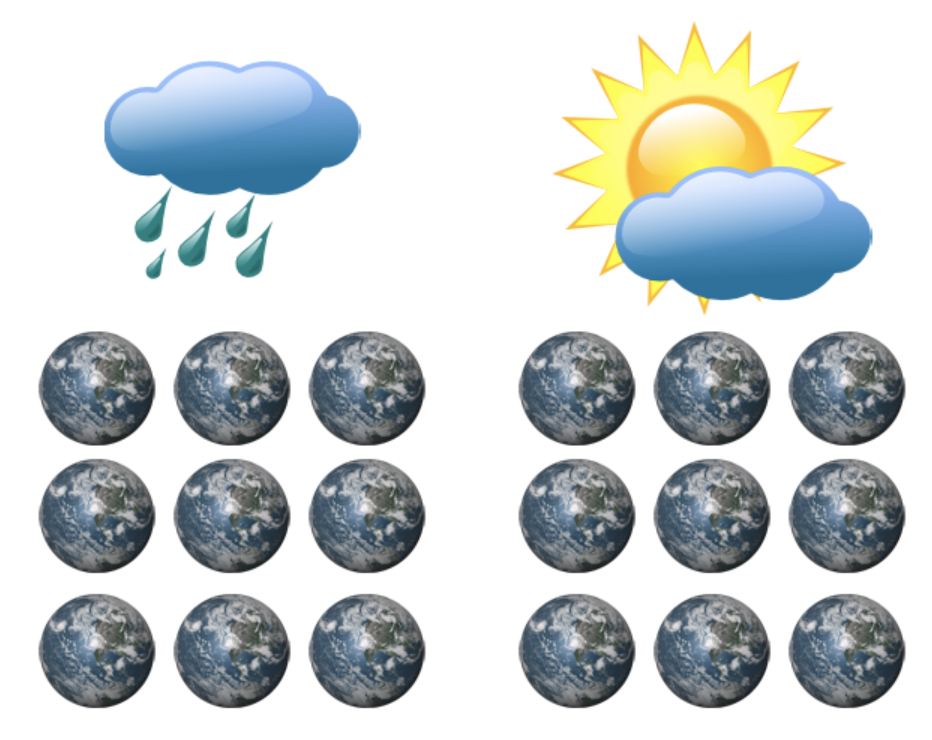
\includegraphics[width=.8\textwidth]{figures/earth_copies}
  \note[item]{But what if you made 100 copies of the earth, and
    arranges the atoms in each one perfectly in exactly the same
    position with the same speed.  would it rain in your location in
    half of them?} 
  \note[item]{Probably it would rain in all of them or none.  if we
    could perfectly model how all the atoms in the atmosphere
    interact, we'd know for sure whether it will rain.} 
  \note[item]{Again, there's no real randomness - probability is just
    a model for the world.} 
\end{frame}

\begin{frame}
  \frametitle{Probability is a Model - Example 3}
  \centering 
  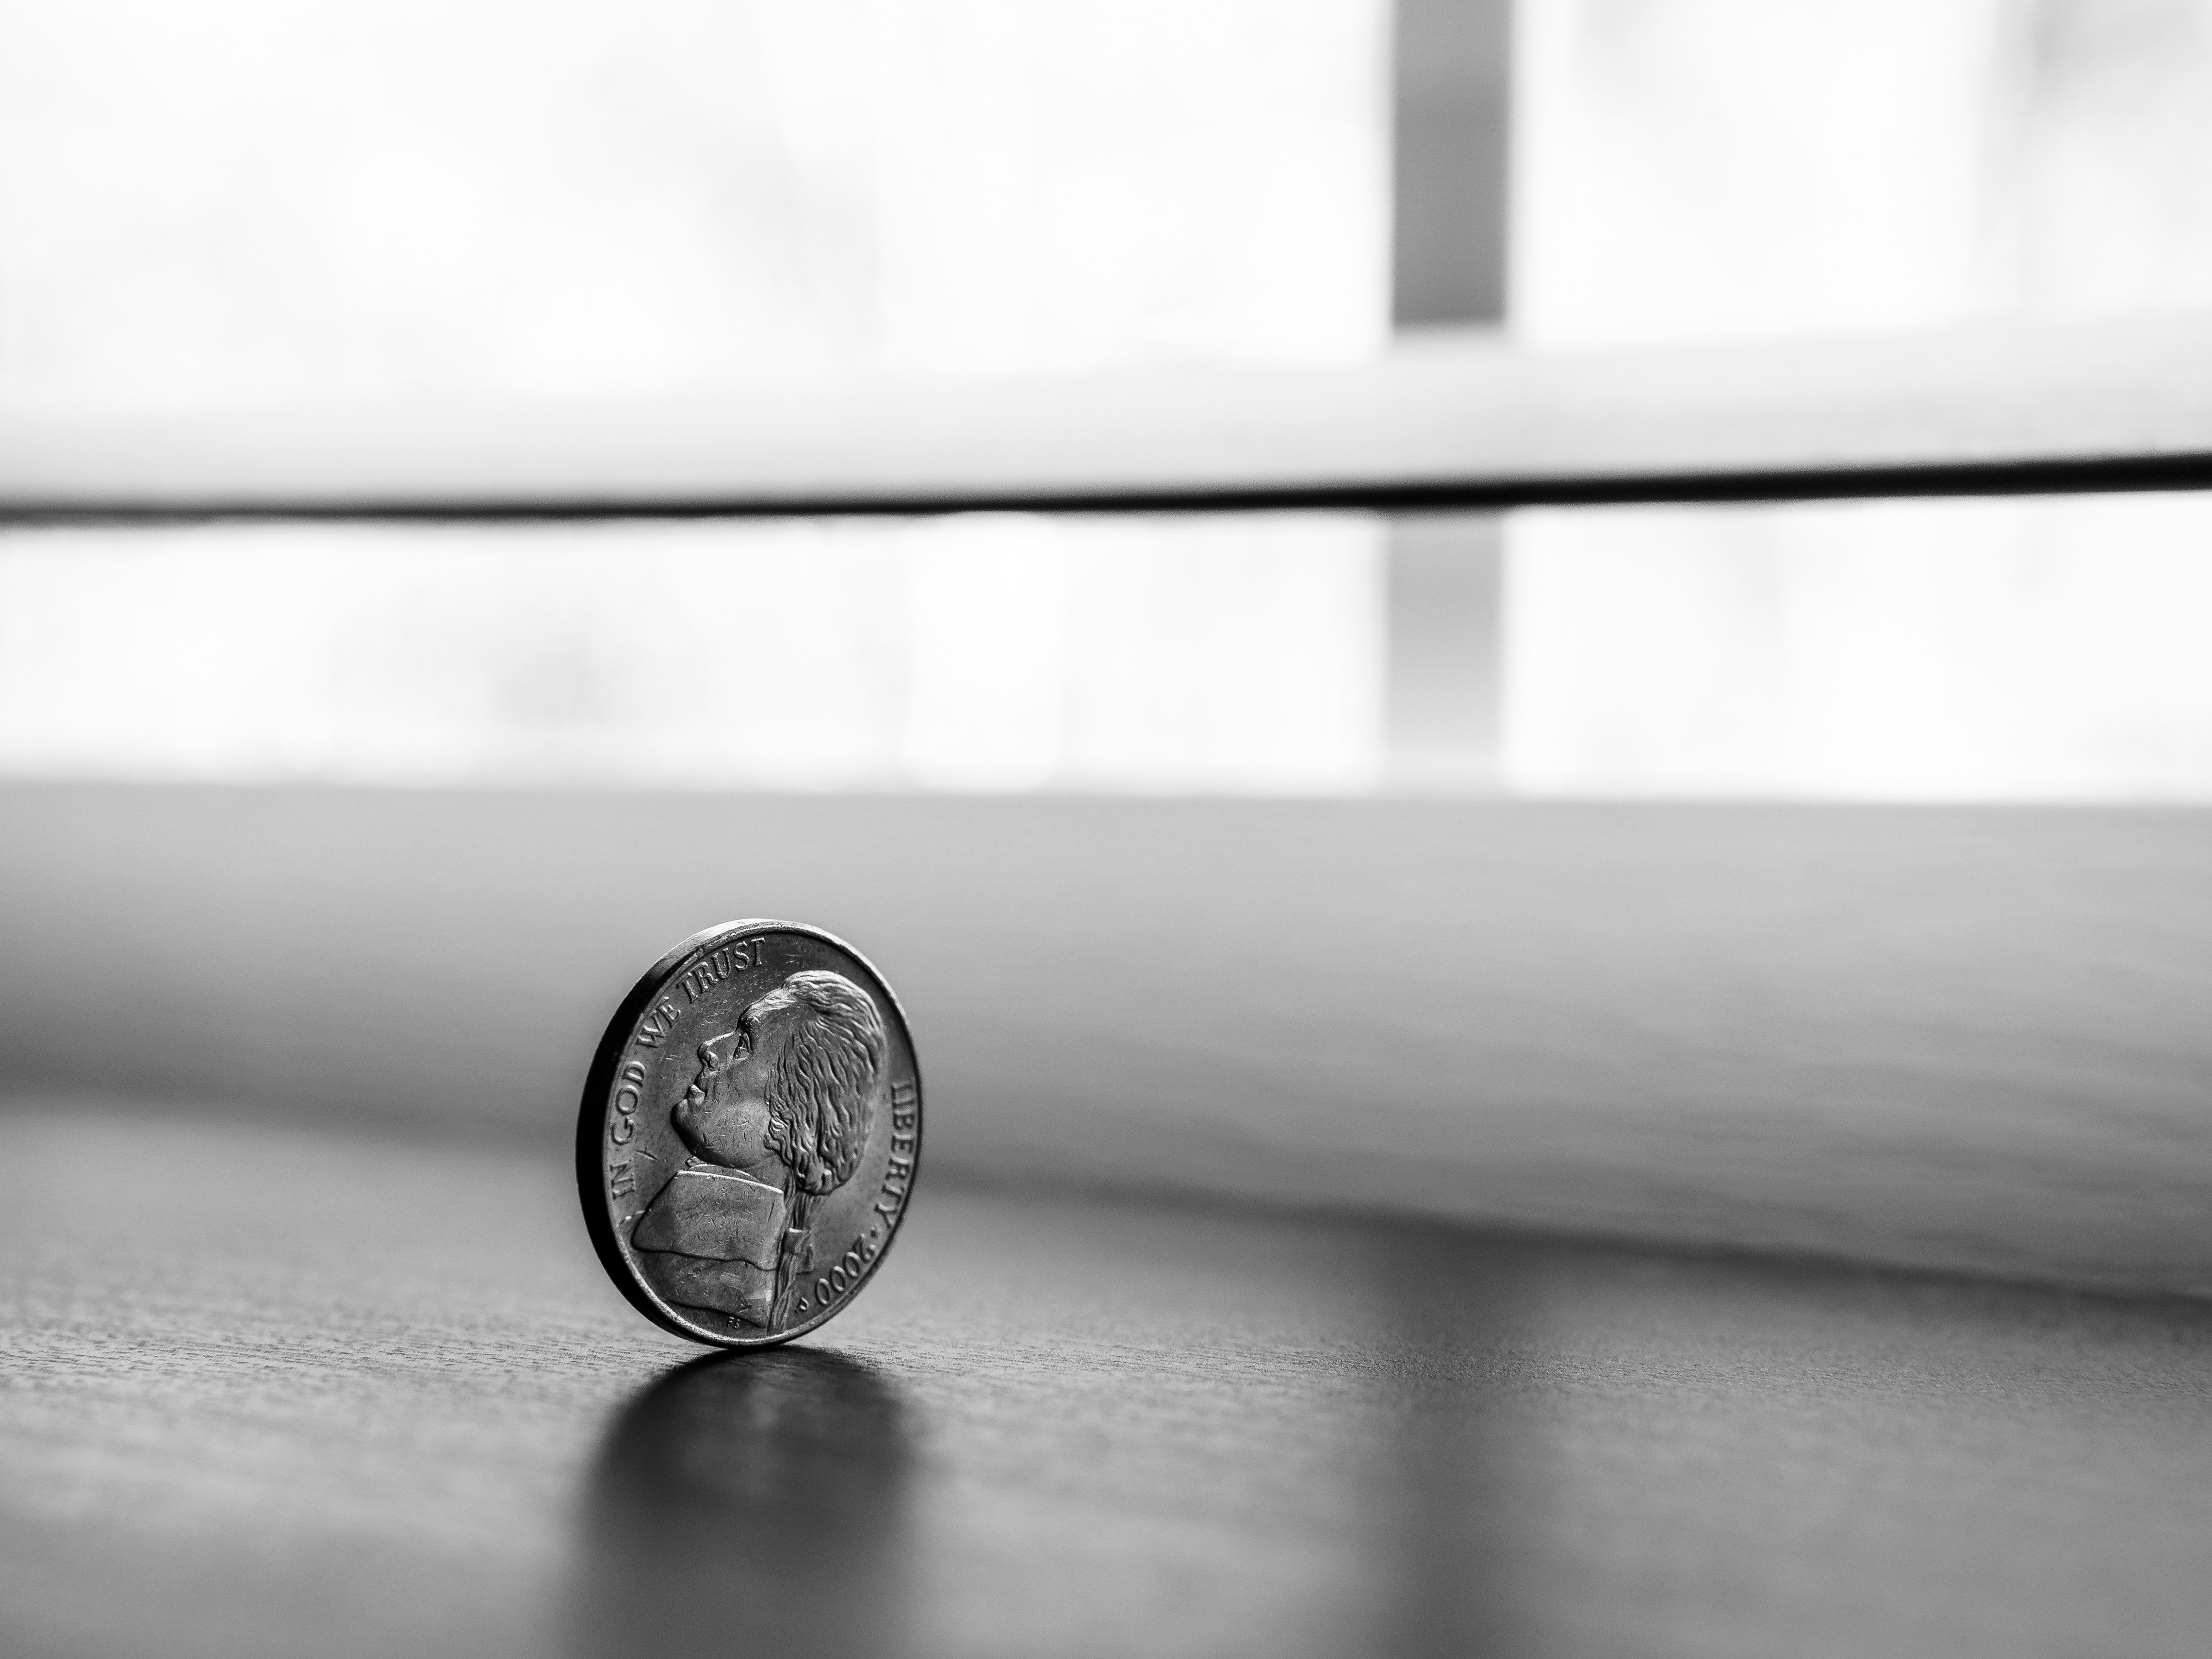
\includegraphics[width=0.8\textwidth]{figures/coin} \\ 
  \note[item]{Finally, what about the most classic random event of all
    - the coin flip.} 
  \note[item]{Everyone knows that a coin lands heads 50\% of the
    time.} 
  \note[item]{But is that true?  What if you could flip the coin in
    exactly the same way each time.} 
  \note[item]{And make sure every single atom in the air was moving in
    exactly the same way.} 
  \note[item]{You would probably find that it lands on the same side
    each time.} 
  \note[item]{Really, the only people who work with true randomness
    are quantum physicists.  The rest of us are using probability as a
    model.} 
\end{frame}


\begin{frame}
  \frametitle{An Axiomatic Approach}
  \note[item]{We already have an intuitive model for probability in
    our heads, but that's not enough to build statistical models - we
    need a mathematically precise system.} 
  \note[item]{How do we create one?  We distill our intuition into a
    small set of axioms.  This is what mathematicians do...} 
  Why take an axiomatic approach?
  \begin{itemize}
  \item Define a minimal set of statements that are consistent with
    the world we observe
  \item Deduce statements that must then be logically entailed
  \end{itemize}

  \note[item]{Suppose that you're rolling die -- you could observe that
    the P(1|2) is just P(1) + P(2).  You could write that down as a fact.}
  \note[item]{\paul{If you kept doing that, you'd end up with a huge
      pile of facts, and you still would not be able to predict the
      probability of a new event. You would have no logical way to
      move from the one fact to another.}} 
  \note[item]{Instead, we need to identify axioms that explain the
    probabilities of many different events. induct up to a higher set
    of principles --  the pieces of the model that we need, that are
    used to repredict to events.}  
  \note[item]{You might find this frustrating -- you might want to
    study this like it is an observational science; counting lions or
    cosmic rays. But, it isn't!}
  \note[item]{Probability is a model, so we're inventing the rules,
    not discovering them.  But if our system reminds us enough of the
    real world, it can be useful.}  
  
  \textit{Thomas Kuhn's} Philosophy of Science

  \begin{itemize}
  \item<1-> Axiomatic statements 
  \item<1-> Intermediate theories 
  \item<1-> Testable hypotheses
  \end{itemize}
\end{frame}


\section{Learnosity: Set Theory Diagnostic Quiz}

% \begin{frame}
%   \frametitle{Learnosity: Set Theory Diagnostic Quiz }
% \note[item]{\paul{Alex, I'm moving this up, because students need some set notation just to read the basic definitions of event spaces, probability measures.}}
% \note[item]{\paul{I think I would find it a bit annoying to click a link - will try to write a short self assessment version in the next slide.}}

%   We presume prior knowledge about the basic algebra of operations on
%   sets. If you are able to reason through this short \underline{ \href{https://en.wikipedia.org/wiki/Algebra_of_sets}{Wikipedia page}}, then you are
%   ready to work on set-based probability and its algebra for the course.
% \end{frame}

\begin{frame}
  \frametitle{Set Theory}
  
  \note[item]{To understand the upcoming definitions, you will need to be familiar
  with basic set theory.  This sequence is a quick review of the set
  operations we will be using most.}
  
  If you already understand the following notation and can solve the
  problem, we recommend that you skip this sequence and go straight to
  the next segment about partitions. 
  
  Notation:
  \note[item]{Probably more notation to add, let's keep an eye out and add as we need it.}
  
  $A$ and $B$ are sets.
  
  \begin{tabular}{c|c}
    union & $A \cup B$ \\
    intersection & $ A \cap B$ \\
    set difference & $A \setminus B$\\
    complement & $A^C$ \\
    empty set & $\emptyset$ \\
  \end{tabular}
  
  
  Simplify the expression: $ (A \cap B) \cup ( B \setminus A) $
\end{frame}


\section{The Set Operations, Part 1}

\begin{frame}
  \frametitle{Visualizing a Set}
  \note[item]{What is a set?  I'm not going to give a precise
    definition, set theory is interesting but it's pretty far down
    into the foundations of mathematics. } 
  \note[item]{What you need to know is that sets contain objects.}
  \note[item]{Imagine a bag, so there's no order inside the set.}
  \note[item]{An object is either in the set or outside.}
  \note[item]{Also, an object can't be in the set twice.  No
    repetition - you're in or you're out.} 
  \begin{columns}
    \begin{column}{0.3\textwidth}
      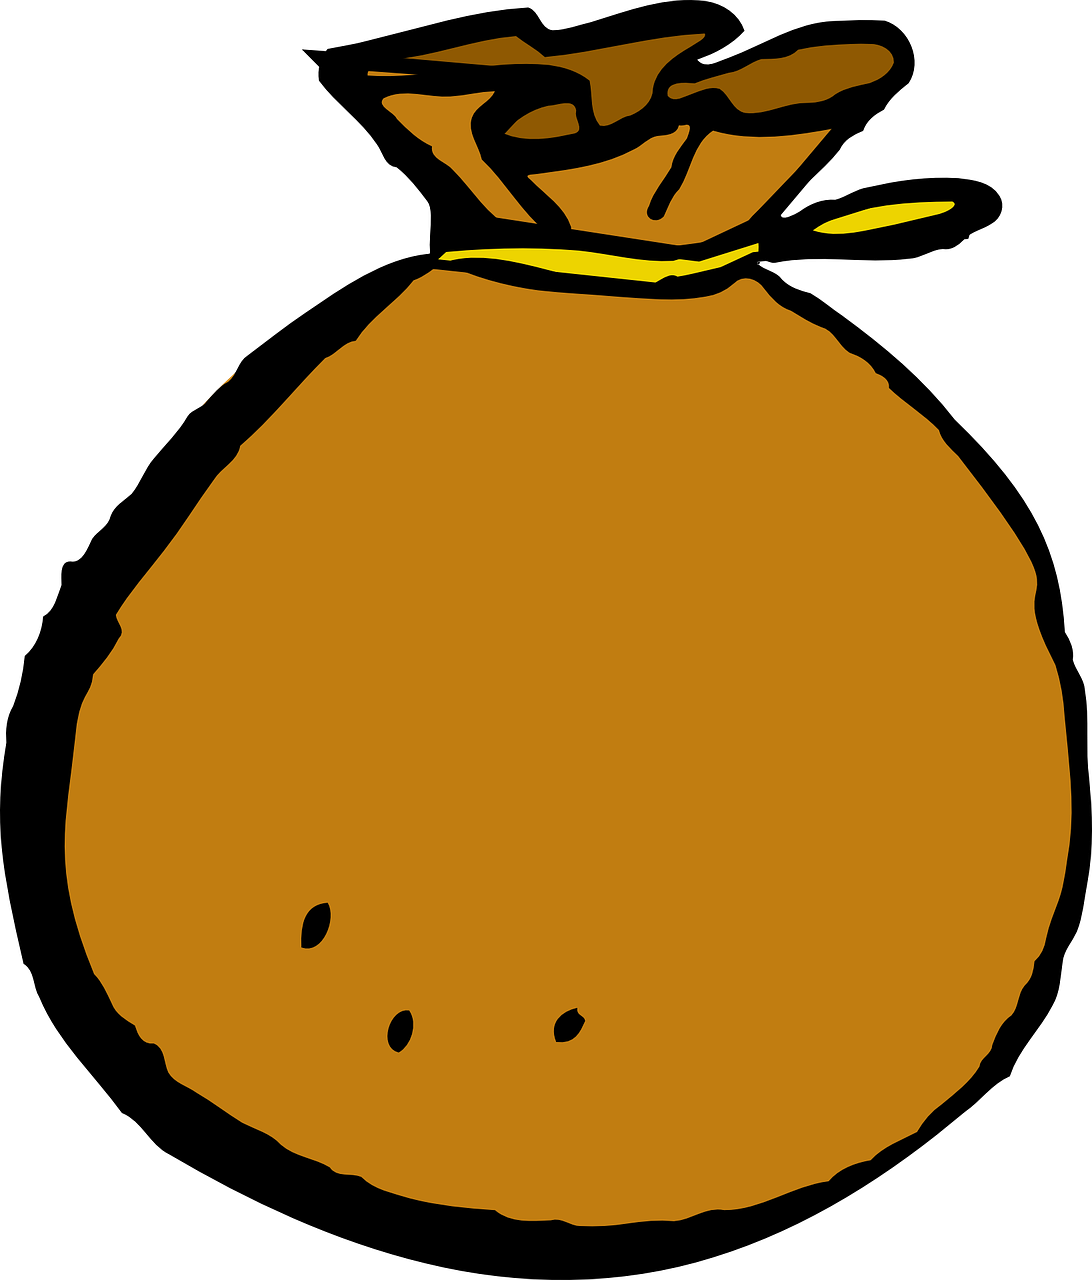
\includegraphics[width=\textwidth]{figures/bag}
    \end{column}
    \begin{column}{0.7\textwidth}  
      \begin{center}
        \begin{itemize}
        \item A set contains objects.
        \item Items don't have an order.
        \item Items can't repeat.
        \end{itemize}        
      \end{center}
    \end{column}
  \end{columns}
\end{frame}


\begin{frame}
  \frametitle{Elements of Sets}
  \note[item]{How do you write down what elements are in a set?}
  \note[item]{To start with, there are two common techniques for building a brand new set}
  \note[item]{First, we can just make a list of all the elements inside curly braces.}
  
  Defining a new set:
  \begin{itemize}
  \item Elements go in curly braces. \note[item]{Let $A = \{1, 2, 3\}$.}
  \item A colon means "such that".  \note[item]{Let $B = \{b : b\text{ is an integer}, 1 \leq b \leq 3\} $}
  \end{itemize}
  
  Specifying elements:
  \begin{itemize}
  \item '$\in$' means '"is an element of."
  \item '$\notin$' means "is not an element of."
  \item '$\emptyset$' means the empty set.
    
    \note[item]{$2 \in A$.  $5 \notin A$}
  \end{itemize}
\end{frame}


\begin{frame}
  \frametitle{Subsets and Supersets}
  \note[item]{A subset is set that's contained inside a set} 
  \note[item]{The larger set is called a superset.} 
  \note[item]{We take every element that's in at least one of the
    sets.} 
  \note[item]{We can write this: $A \subseteq B$ if for every $x \in
    A, x \in B$ } 
  \note[item]{Most of the time, when we say subset, we mean that A is
    inside B but A could be exactly the same as B.} 
  \note[item]{If you ever really need to say that A is a subset and
    actually smaller, you can add a slash through the bottom line.
    that's called a strict subset or proper subset.} 
  
  \begin{minipage}[t]{0.5\textwidth}
    \vspace{0pt}
    $ A = \{1,2\}, \ B = \{1,2, 3,4\}$
    
    \vspace{1cm}
    Subset: $A \subseteq B$
    
    \vspace{1cm}
    Strict Subset: $A \subsetneq B$
  \end{minipage}%
  \hfill
  \begin{minipage}[t]{0.5\textwidth}
    \vspace{-5pt}
    \center  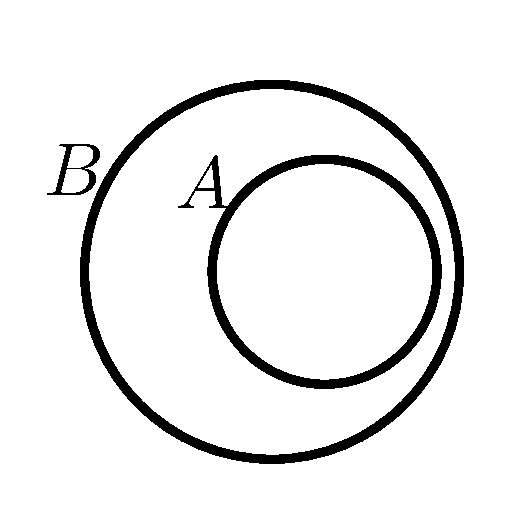
\includegraphics[width=\linewidth]{figures/subset}
  \end{minipage}  
\end{frame}

\begin{frame}
  \frametitle{Set Union}
  \note[item]{A set union means we're merging sets together}
  \note[item]{We take every element that's in at least one of the sets.}
  \note[item]{We can write this: $\{ x : x \in A \text{ OR } x \in B\}$ }
  \note[item]{Remember that: Union means OR}
  \note[item]{In this case, $ = \{1,2,3,4\}$}

  \begin{minipage}[t]{0.5\textwidth}
    \vspace{0pt}
    $ A = \{1,2,3\}, \ B = \{3,4\}$
    
    Union is $A \cup B$
  \end{minipage}%
  \hfill
  \begin{minipage}[t]{0.5\textwidth}
    \vspace{-5pt}
    \center  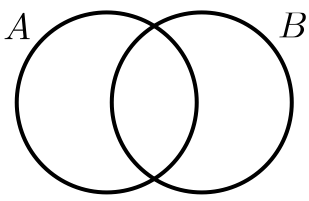
\includegraphics[width=\linewidth]{figures/union}
  \end{minipage}  
\end{frame}


\begin{frame}[t]
  \frametitle{Properties of Unions}

  \begin{itemize}
  \item Symmetry: $A \cup B = B \cup A$
  \item Association: $(A \cup B) \cup C = A \cup (B \cup C)$
  \item $A \cup A = A$
  \item $A \cup \emptyset = A$
  \end{itemize}
  \note[item]{I don't want to prove these, because we have a lot to cover.   they all follow very quickly from properties of or, as a logical operator. I'll prove one to give you an example}
  \note[item]{$x \in (A \cup B) \cup C \Leftrightarrow x \in (A \cup B) \text{ OR } x \in C$}
  \note[item]{$\Leftrightarrow x \in A \text{ OR } x \in B \text{ OR } x \in C $ (I don't need parentheses because order doesn't matter for OR.)}
  \note[item]{$\Leftrightarrow x \in A \text{ OR } x \in (B \cup C) \Leftrightarrow x \in A \cup ( B \cup C ) $}
  \note[item]{Like I said, we're really down in the foundations.}
\end{frame}

\section{The Set Operations, Part 2}

\begin{frame}
  \frametitle{Set Intersection}
  \note[item]{A set intersection means we want only the common elements}
  \note[item]{We take every element that's in BOTH of the sets.}
  \note[item]{We can write this: $\{ x : x \in A \text{ AND } x \in B\}$ }
  \note[item]{Remember that: Intersection means AND}
  \note[item]{In this case, $ = \{3\}$}
  \note[item]{What if there is nothing in the intersection at all?}
  \note[item]{If $X \cap Y = \emptyset$ then X and Y are disjoint.}
  
  \begin{minipage}[t]{0.5\textwidth}
    \vspace{0pt}
    $ A = \{1,2,3\}, \ B = \{3,4\}$
    
    Intersection is $A \cap B$
    
    \vspace{3cm}
    Two sets are \textit{disjoint} if their intersection is empty.
  \end{minipage}%
  \hfill
  \begin{minipage}[t]{0.5\textwidth}
    \vspace{-5pt}
    \center  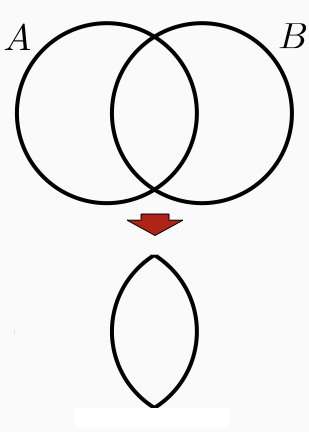
\includegraphics[width=\linewidth]{figures/intersection}
  \end{minipage}  
\end{frame}


\begin{frame}
  \frametitle{Properties of Intersections}
  \begin{itemize}
  \item Symmetry: $A \cap B = B \cap A$
  \item Association: $(A \cap B) \cap C = A \cap (B \cap C)$
  \item $A \cap A = A$
  \item $A \cap \emptyset = \emptyset$
  \end{itemize}
\end{frame}


\begin{frame}
  \frametitle{Distributing Union and Intersection}
  
  \begin{minipage}[t]{0.6\textwidth}
    \vspace{0pt}
    
    $A \cup (B \cap C) = (A \cup B) \cap (A \cup C)$
    
    \vspace{2cm}
    $A \cap (B \cup C) = (A \cap B) \cup (A \cap C)$
    
  \end{minipage}%
  \hfill
  \begin{minipage}[t]{0.4\textwidth}
    \vspace{-5pt}
    \center  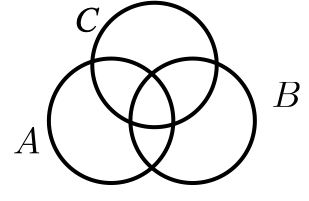
\includegraphics[width=\linewidth]{figures/abc}
  \end{minipage}  
  
\end{frame}


\begin{frame}
  \frametitle{Set Difference}
  \note[item]{A set difference means we want the elements in one set but NOT the other.}
  \note[item]{It's like subtracting one set from another.}
  \note[item]{We can write this: $\{ x : x \in A \text{ AND } x \notin B\}$ }
  \note[item]{In this case, $ = \{1,2\}$}
  
  \begin{minipage}[t]{0.5\textwidth}
    \vspace{0pt}
    $ A = \{1,2,3\}, \ B = \{3,4\}$
    
    Difference is $A \setminus B$
    
    
  \end{minipage}%
  \hfill
  \begin{minipage}[t]{0.5\textwidth}
    \vspace{-5pt}
    \center  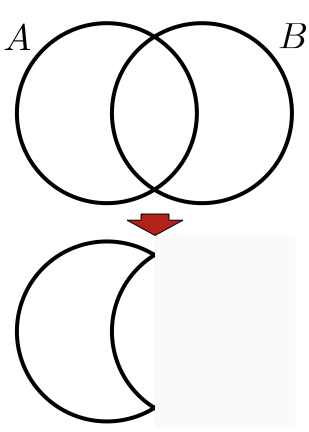
\includegraphics[width=\linewidth]{figures/difference}
  \end{minipage}  
\end{frame}



\begin{frame}
  \frametitle{Distributing Set Difference}
  \note[item]{There are also ways to distribute set differences over the other operations.}
  \note[item]{It can be hard to remember these all at once, but let me highlight this first one, which we're definitely going to use.}


  \begin{minipage}[t]{0.6\textwidth}
    \vspace{0pt}
    
    $A \cap (B \setminus C) = (A \cap B) \setminus C$
    
    \vspace{1cm}
    $C \setminus (A \cap B) = (C\setminus A) \cup (C \setminus B)$
    
    \vspace{1cm}
    $C \setminus (A \cup B) = (C\setminus A) \cap (C \setminus B)$
    
  \end{minipage}%
  \hfill
  \begin{minipage}[t]{0.4\textwidth}
    \vspace{-5pt}
    \center  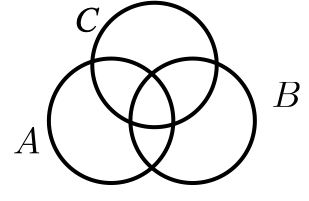
\includegraphics[width=\linewidth]{figures/abc}
  \end{minipage}   
\end{frame}




\begin{frame}
  \frametitle{Set Complement}
  \note[item]{We we're doing probability theory, we're going to do all of our work inside a big set, which we call the sample space $\Omega$.  Every set will be a subset of $\Omega$.}
  \note[item]{In this case, we have a special name for everything not in a set, A - we call it the complement}
  \note[item]{\paul{Shade in complement}}
  \note[item]{The complement is just a set difference, $\Omega \setminus A$}
  \note[item]{In this case, $=\{4,5\}$}
  
  \begin{minipage}[t]{0.6\textwidth}
    \vspace{0pt}
    $\Omega$ - ALL objects of interest.
    
    $ A = \{1,2,3\}, \ \Omega = \{1, 2, 3,4,5\}$
    
    Complement: $A^C = \Omega \setminus A$
    
    
    \vspace{1cm}
    Properties:
    \begin{itemize}
    \item  $A^C \cup A = \Omega$
    \item $A \setminus B = A \cap B^C$
    \end{itemize}
    
    \note[item]{$A \setminus B  = (A \cap \Omega) \setminus B = A \cup ( \Omega \setminus B) = A \cup B^C$}
    
  \end{minipage}%
  \hfill
  \begin{minipage}[t]{0.4\textwidth}
    \vspace{-5pt}
    \center  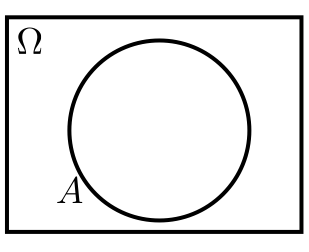
\includegraphics[width=\linewidth]{figures/complement}
  \end{minipage}   
\end{frame}


\section{Set Partitions}

\begin{frame}
  \frametitle{Set Partitions}
  \begin{block}{Definition 1.1.12: \textit{partition}}
    A set of sets $A_{1}, A_{2}, \dots, A_{n}$ is a \textit{partition} of set $S$, if $A_{1}, A_{2}, \dots, A_{n}$ are nonempty and
    pairwise disjoint, and if $S = A_{1} \cup A_{2} 
    \cup \cdots \cup A_{n}$.
  \end{block}
  
  \begin{center}
    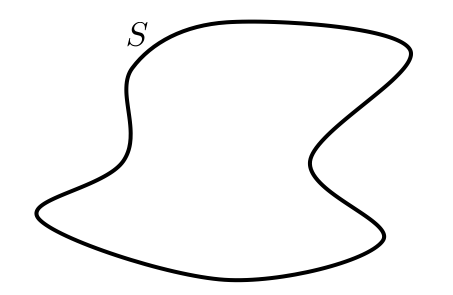
\includegraphics[width=0.7\textwidth]{./figures/set_for_partition}
  \end{center}
  
  \note[item]{While we're talking about sets, there's an idea that's really useful, which is dividing a set up into a partition.  Let's read exactly what a partition is... }
  \note[item]{Here's a set $S$ - how do I create a partition?  I will draw in some sets.  each one has to be completely inside $S$, and they can't overlap at all.  And I have to make sure I cover all of $S$.}
\end{frame}


\begin{frame}[t]
  \frametitle{Partition Rule 1}
  Given a set $A$ and another set $B$, a partition of $A$ is...
  \center 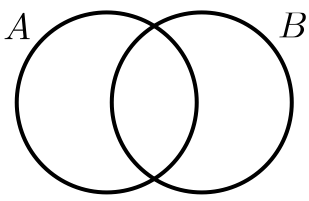
\includegraphics[width=0.5\textwidth]{./figures/ab}
  
  \note[item]{Can you see the partition?  Here's one piece, and here's the other.}
  \note[item]{This one is A minus B, this one is the intersection.  Let's quickly prove it...}
  \note[item]{$A  = A \cap (B \cup B^C) = (A \cap B) \cup (A \cap B^C)  = (A \cap B) \cup (A \setminus B)$}
\end{frame}


\begin{frame}[t]
  \frametitle{Partition Rule 2}
  Given a set $A$ and another set $B$, a partition of $A \cup B$ is...
  \center 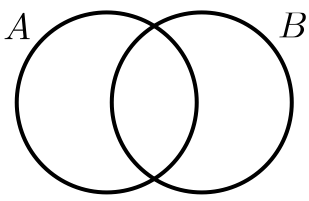
\includegraphics[width=0.5\textwidth]{./figures/ab}
  
  \note[item]{Here's a slightly harder problem, what if we want to partition the entire union?}
  \note[item]{This time, we can break it apart into 3 pieces.  Same as last time, plus also B minus A.}
  \note[item]{Let's quickly prove it...}
  \note[item]{Let's just apply the previous relationship twice!}
  \note[item]{$A \cup B   = (A \cap B) \cup (A \setminus B) \cup (A \cap B) \cup (B \setminus A) $}
  \note[item]{Guess what, A intersect B is in there twice.  if you take a union of a set with itself, you get the same set, so we can just remove one of them and we're done.}
\end{frame}



\begin{frame}
  \frametitle{Call to Reading}
  \begin{itemize} 
  \item Chapter 1, from page 3 to the top of page 8, stopping before \textit{Theorem 1.1.1}
  \end{itemize}
\end{frame}


%\begin{frame}
%  \frametitle{Probability is Reasoning under Uncertainty}
%
%  \begin{exampleblock}{Example}
%    Some example here
%  \end{exampleblock}
%\end{frame}



\section{Probability Spaces}

\begin{frame}
  \frametitle{Fundamental Components of Probability Space}
  \begin{block}{A Probability Space}
    \begin{itemize}
    \item A \textbf{sample space}, denoted as $\Omega$, is the
      collection of \textit{all} possible outcomes.
    \item An \textbf{event space}, denoted as $S$, is made up of sets of outcomes.
    \item A \textbf{probability measure} is a function that maps
      events to numbers in $[0,1]$.
    \end{itemize}
    % include squiggly picture
  \end{block}
  \note[item]{To build statistical models, we need a mathematical description of probability.}
  \note[item]{We need to take our intuition for what a system with uncertainty means, and encode it into a mathematical object.  that object will be what we call a probability space. }
\end{frame}

\begin{frame}
  \frametitle{Sample Spaces}
  \note[item]{Let's start with the sample space.  where do we get the sample space?  well we have to design it to represent the real world.  Let's give some examples.}
  Choosing sample space $\Omega$ to represent...
  \begin{itemize}
    \setlength{\itemsep}{14pt}%
  \item A die % which is discrete
  \item A dartboard % which is continuous
  \item A survey of 5 U.S. senators
  \item A spoken conversation
  \end{itemize}
  \note[item]{A die  -- $\{1, 2, 3, 4, 5, 6\}$}
  \note[item]{A dartboard -- $\{(x,y) \text { such that } x^{2} + y^{2} \leq 1\}$}
  \note[item]{A survey of 5 U.S. senators -- $\{ S: S \subseteq Senators, |S| = 5 \}$ This is
      not individual people, it's a set of sets! there are 100 choose 5 outcomes. }
  \note[item]{Suppose you're doing language translation --  $\{ (w_1, w_2,...,w_k) : w_1,w_2,...w_k \text{are words} \} $.}
    \note[item]{Question: can you apply a probability measure directly to the set of outcomes?  unfortunately, no.  for simple ones you can, but what about the dartboard. there are an infinite number of locations, and the probability of each one is just zero.  but a function that's zero everywhere doesn't help us model this.}

\end{frame}


\begin{frame}
  \frametitle{Events}
  An event is a set of outcomes.
  
  \begin{itemize}
  \item Rolling an even number. \note[item]{$\{2,4,6\}$ }
    % \item Rolling a 4. \note[item]{ $\{4\}$ }
  \item Hitting a bullseye. \note[item]{$\{(x,y) \text{ such that } x^2 + y^2 \leq .05\}$}
    % \item Getting five dirty hippies in your survey: $\big\{ \{\text{Celeste, Dawn, Harmony, Indigo, Marley}\}, $ 
    %   $\{\text{Mike Rivera, Dawn, Harmony, Karma, Leaf}\}, ... \big\}$
  \item Starting a sentence with 'Um'.
   
  \end{itemize}
\end{frame}

 
\begin{frame}
  \frametitle{Forming New Events}
  
  \begin{columns}
    \begin{column}{0.3\textwidth}  
      \begin{center}
        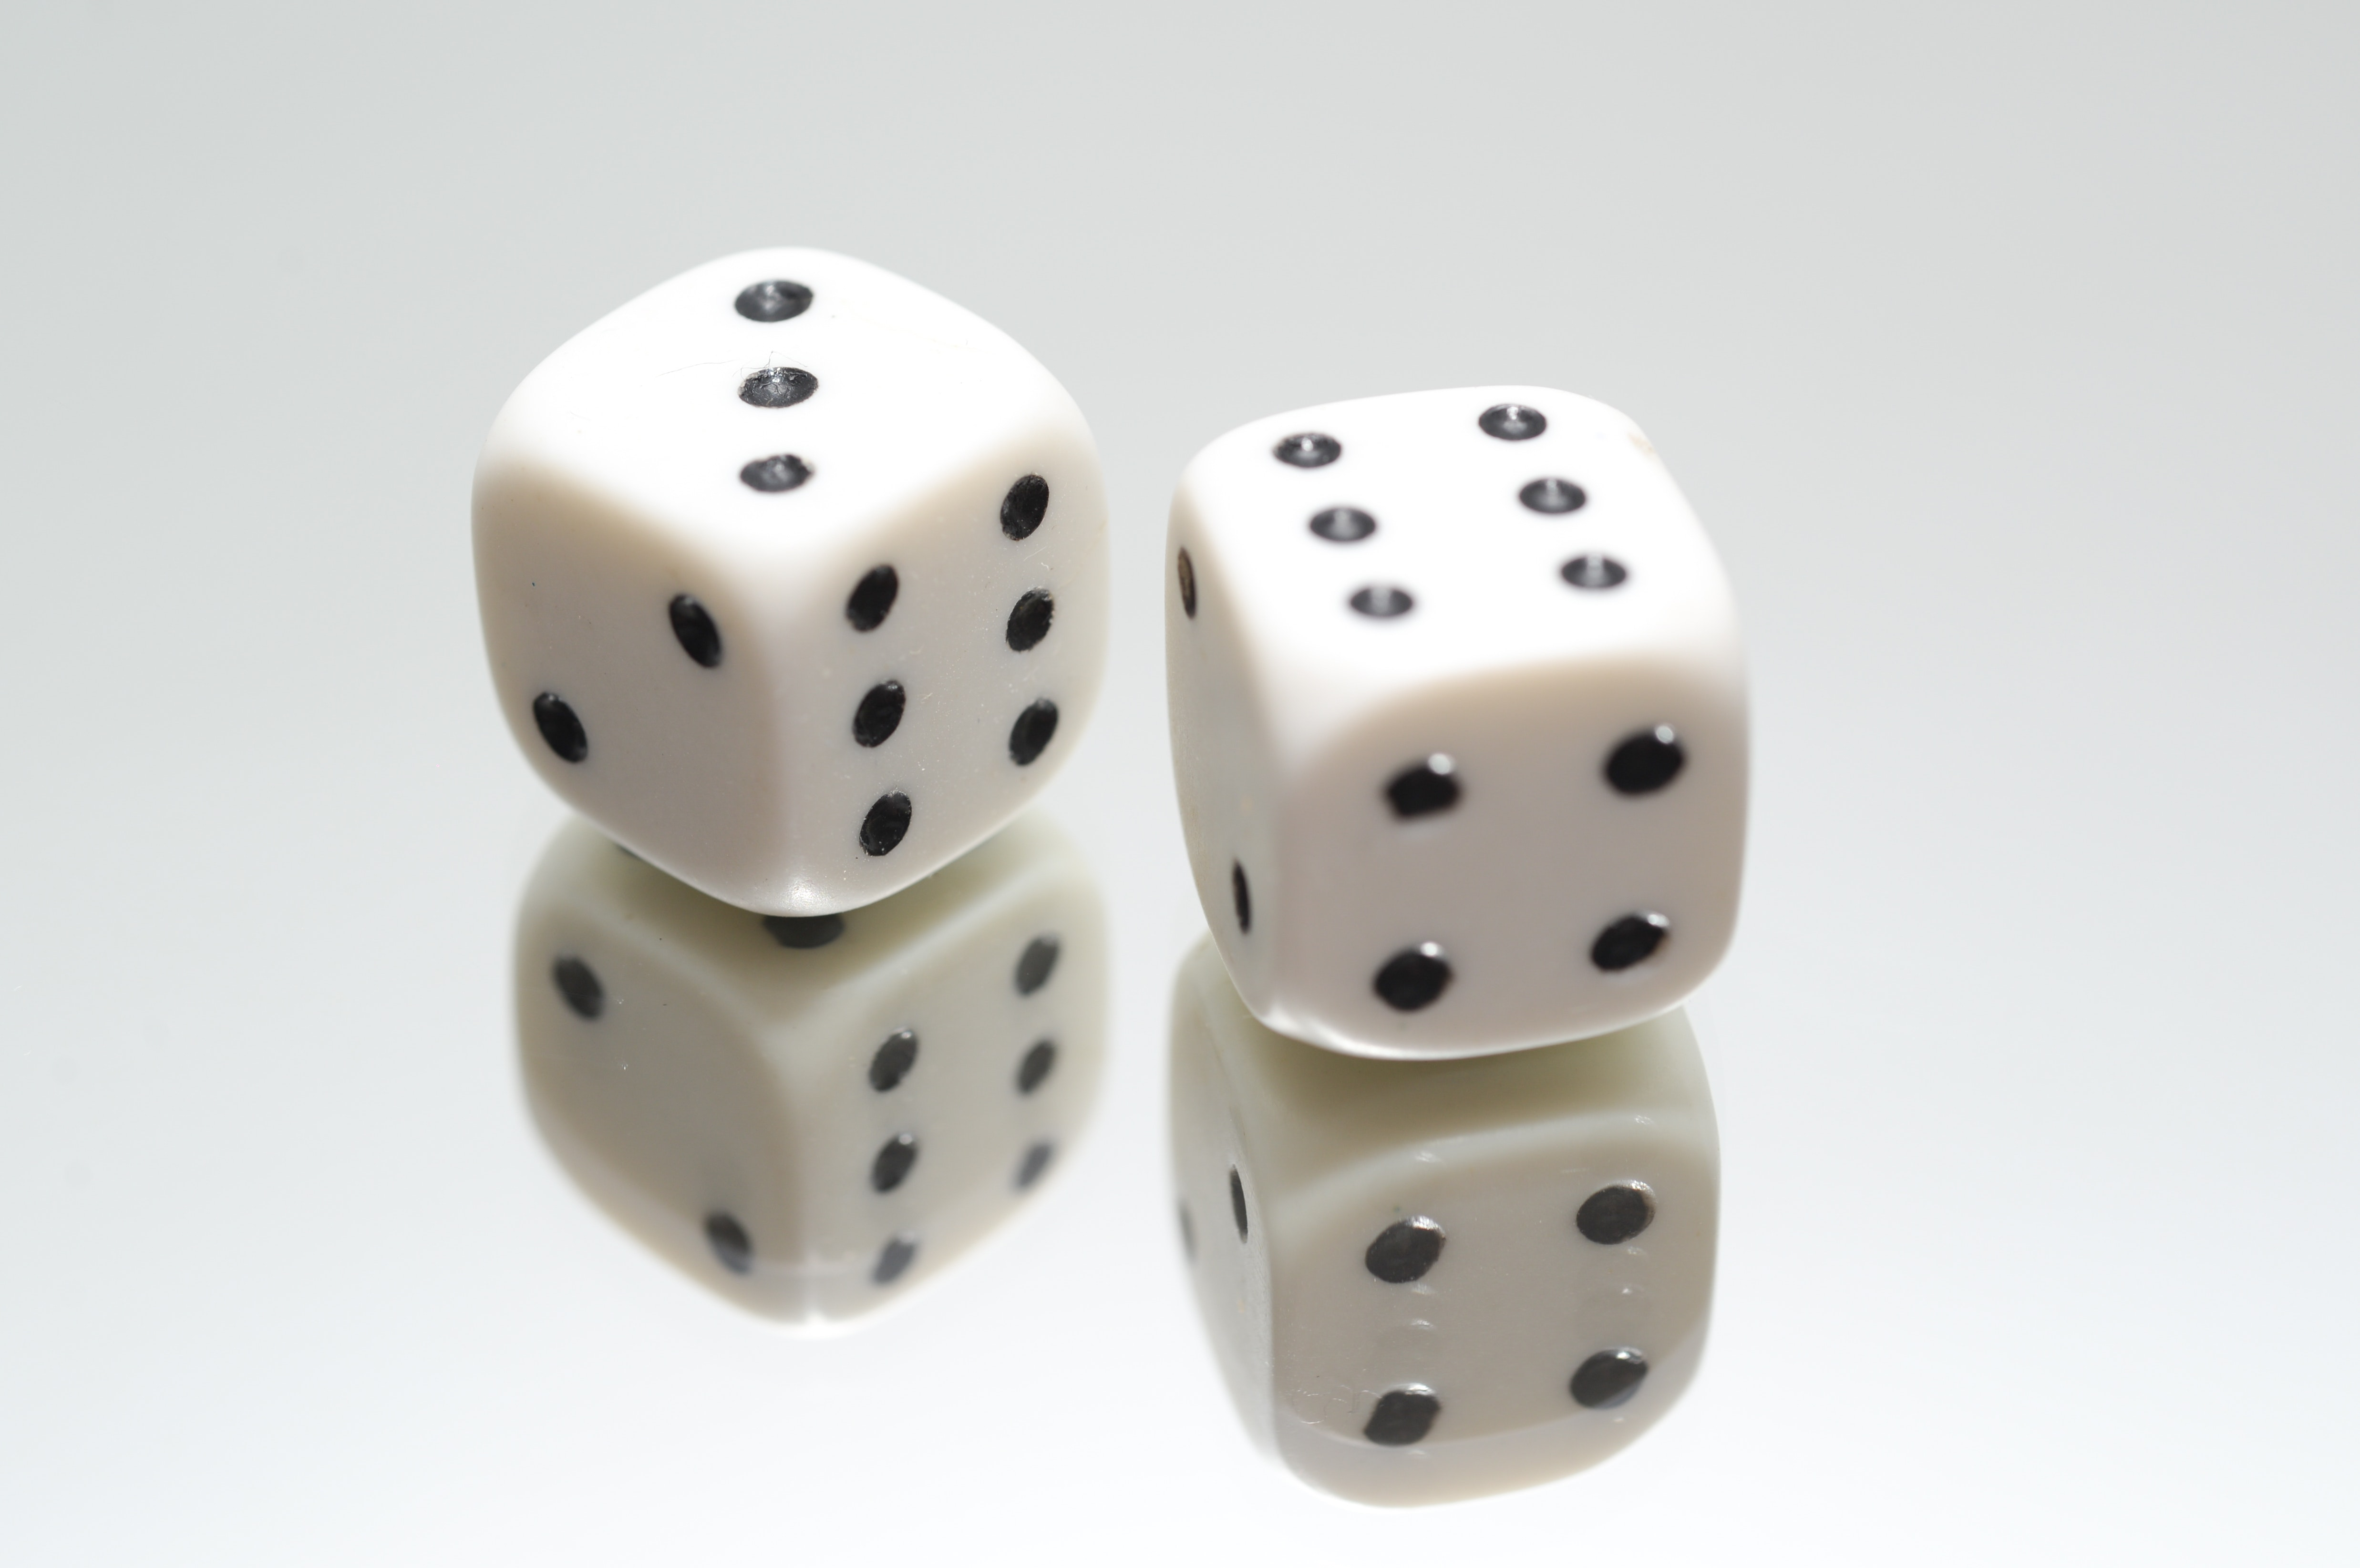
\includegraphics[width=\textwidth]{figures/dice}
      \end{center}
    \end{column}
    
    \begin{column}{0.7\textwidth}
      $A = \{1,2\}, B = \{2,4,6\}$ 
      \vspace{.5cm}
      \note[item]{Because events are sets, we can combine them with
        set operations to make new events.  Let's think about what
        those operations mean.} 
      \note[item]{Here's two events for the simple example of a die roll}
      \note[item]{First, think about how you would write down the
        event A OR B?  that is, either A occurs or B occurs.} 
      \note[item]{Well, that means that the outcome that occurs must
        be in at least one of A or B, so it must be in their union.
        When you see a union, think OR.} 
      
      
      \begin{itemize}
  \setlength\itemsep{1em}
      \item A OR B:
      \item A AND B:
      \item NOT A:
      \end{itemize}
      
    \end{column}
  \end{columns}  
\end{frame}



\begin{frame}
  \frametitle{Event Spaces}
  \begin{block}{Intuition for an event space}
    \note[item]{Now we have a bunch of events, and we want to group them
      all together and call that an event space.} 
    \note[item]{That seems like a simple idea, right?  But when you read
      the textbook, you might have wondered, why is this so complicated?
      well, it gets fairly technical, but it turns out that there are
      sometimes sets of outcomes that we have to exclude from the event
      space.  These are called non measurable.} 
    
    \begin{itemize}
    \item $S$ represents all possible events 
      
    \item However, there are technical reasons that some sets of outcomes must be excluded (non-measurable).  
      
    \end{itemize}
  \end{block}
  
  
  \note[item]{So Mathematicians said: we can't put all possible sets
    in the event space, let's just make sure that any set we need for
    a regular analysis is in there.  So they came up with a list of
    guarantees and the technical term for these is a
    $\sigma$-algebra)} 
  
  \note[item]{You can think of this as making sure that any way you
    can combine events together, the answer will always be an event,
    so it will have a probability.  You can't accidentally fall out of
    the event space. } 
  
  \textbf{Requirements for a $\sigma$-algebra}
  \begin{itemize}
  \item Nonempty: $S \neq \emptyset$
  \item Closed under complements: If $A \in S$ then $A^C \in S$
  \item Closed under countable unions: if $A_1,A_2,... \in S$ then $A_1 \cup A_2 \cup ... \in S$
  \end{itemize}
\end{frame}




\begin{frame}
  \note[item]{Finally, the last element is the probability measure itself.  To be a valid probability measure, a function has to satisfy three properties.}
  \note[item]{Where do these come from?  We're building a model here.  we're taking properties from our intuition and trying to write them down using math.}
  \note[item]{First, there are no negative probabilities.  that just makes sense to us, right?  what would a negative probability mean?}
  \note[item]{Next, the probability of the entire outcome space is 1.  That should make sense too, because some outcome must happen. the state of the world will be something.}
  \note[item]{Finally, the addition rule.  Probabilities add up when we combine events, as long as they are disjoint.  The probability of rolling a 1 or a 2 is the probability of rolling a 1 plus the probability of rolling a 2.  But in standard probability theory that even works for a countably infinite set of disjoint events.}
  \note[item]{What's the probability that the sun goes supernova someday?  well, you can add the probability for today, plus the probability for tomorrow, and on forever.}
  \frametitle{Probability Measure}
  \begin{block}{Definition of a probability measure}
    A function $P: S \rightarrow \mathbb{R}$ is a
    probability measure if:
    \begin{itemize}
    \item \textbf{Axiom 1.} There are no negative probabilities:
      $\forall A \in S: P(A) \geq 0$
    \item \textbf{Axiom 2.} The probability that \textit{some} outcome occurs is one:
      $P(\Omega) = 1$
    \item \textbf{Axiom 3.} Probabilities "add up": If $A_1,A_2,...$ is a countable set of disjoint events, then
      $P(A_1 \cup A_2 \cup ... ) = \sum_{i} P(A_{i})$
    \end{itemize}
  \end{block}
\end{frame}





\begin{frame}
  \note[item]{Looking back at this list of axioms, you might wonder, why only 3?}
  \note[item]{What happens if we take a union, but events aren't disjoint?  Don't we need a property about that?}
  \note[item]{That is an important property, but we don't need it here, because we can derive it from just these three.   That's what we'll do next. }
  \note[item]{\paul{Lot of talking for this slide, I wonder if we can break it into multiple.}}
  \frametitle{Probability Measure}
  \begin{block}{Definition of a probability measure}
    A function $P: S \rightarrow \mathbb{R}$ is a
    probability measure if:
    \begin{itemize}
    \item \textbf{Axiom 1.} There are no negative probabilities:
      $\forall A \in S: P(A) \geq 0$
    \item \textbf{Axiom 2.} The probability that \textit{some} outcome occurs is one:
      $P(\Omega) = 1$
    \item \textbf{Axiom 3.} Probabilities "add up": If $A_1,A_2,...$ is a countable set of disjoint events, then
      $P(A_1 \cup A_2 \cup ... ) = \sum_{i} P(A_{i})$
    \end{itemize}
  \end{block}
\end{frame}



\section{Learnosity Concept Check}


\begin{frame}
  \frametitle{}
  \note[item]{\paul{I'm trying to write one that starts by defining
      the outcomes, so there's no flexibility in choosing Omega, and
      also a clear distinction between outcomes and events.}} 
  \note[item]{\paul{I like this one better than the ones below, let me know what you think.}}
  You run an experiment in which you flip 3 coins, and each one lands
  heads or tails.  Your sample space can be written: $\{HHH, HHT, HTH,
  HTT, THH, THT, TTH, TTT\}$. Assume all outcomes have equal
  probability. 
  \begin{itemize}
  \item  (Assuming that you include all possible sets) what is the size of the event space?
\item  How many outcomes are in the event that the first coin lands heads?
\item If A is the event that the first coin lands heads, and B is the
  event that the second and third coin land the same way, what is the
  probability of $A \cup B$ 
\end{itemize}


\end{frame}


\begin{frame}
  \frametitle{A Single Coin Example} 
  \begin{exampleblock}{A fair coin}
    Suppose that a coin is fair. Then, let $H$ be the event that the
    coin comes up ``heads'' and $T$ be the event that it comes up
    ``tails.''
    \begin{itemize} 
    \item What is the sample space, $\Omega$? 
    \item What is the probability measure for any single outcome,
      $\omega$? 
    \item How many outcomes are in  event $H$? 
    \item If you apply the probability measure to each outcome in $H$, what do you compute for $P(H)$?
    \end{itemize}
  \end{exampleblock}
  
  \note[item]{\paul{bit messy here... we're defining events before defining outcomes, and there is flexibility in how outcomes are defined}}
  \note[item]{\paul{when we say a coin is fair, that's a constraint on the probabilities of certain events.}}
\end{frame}

\begin{frame}
  \frametitle{Learnosity: A Double Coin Example}
  \begin{exampleblock}{Two fair coins} 
    Suppose that you have two coins, and both are fair. Then, let $H$
    be the event that when you toss both coins, at least one comes up
    heads.
    \begin{itemize} 
    \item What is the sample space, $\Omega$? 
    \item What is the probability measure for any particular outcome,
      $\omega$? Are any of these more likely than any other?  
    \item How many outcomes are in
      event $H$? 
    \item If you apply the probability measure to each outcome in $H$, what do you compute for $P(H)$?
    \end{itemize} 
  \end{exampleblock}
  \note[item]{\paul{also having second thoughts about this one.  It might be very intuitive, but we haven't given any machinery to solve for the probability of each outcome.}}
\end{frame}


\section{Reading: Properties of Probability}

\begin{frame}
  \frametitle{Reading: Properties of Probability}
  
  Read page 8 through the end of page 10.
\end{frame}



\section{Deriving Properties of Probability}



\begin{frame}
  \frametitle{A Helpful Analogy}
  
  \center \textbf{Probability $\Longleftrightarrow$ Area}
  
      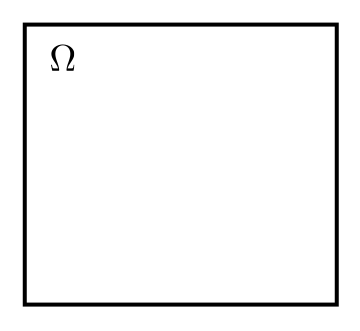
\includegraphics[width=.6\textwidth]{figures/sample_space}
  
  \note[item]{The amazing thing about probability is that with just 3
    axioms, you can prove all the other properties that you expect
    based on your intuition.  But it can be tough to find a solution
    just by staring at equations.} 
  \note[item]{Here's an analogy that may help you.}
  \note[item]{Probabilities are a lot like areas.  Actually, area is
    also a type of measure in mathematics - most of the structure is
    the same.} 
  \note[item]{If you just have a few events, it can help to draw them
    as areas.  That's not a proof, but it can give you an idea of how
    they behave.} 
  \note[item]{Let's think about the sample space as a square
    dartboard.  We'll define its area to be 1.  I'm really bad at
    darts so every point is just as likely as any other point.} 
  \note[item]{An event is some shape on the dartboard.  so the
    probability that the dart lands in the shape is its area. A
    picture like this can help you figure out a tricky proof.} 
\end{frame}


\begin{frame}
  \frametitle{The Subset Subtraction Rule}
  Given $A,B \in S$, $A \subseteq B$.  Compute $P(B\setminus A)$.
  
  Ex: A = being over 7', B = being over 6'.


   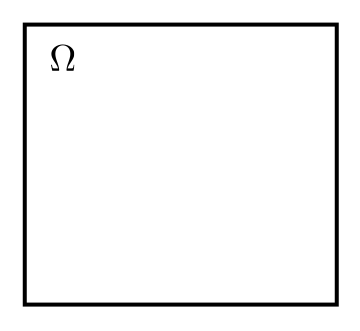
\includegraphics[width=.6\textwidth]{figures/sample_space}
   
   \note[item]{Let's start with a simple property, if we assume that
     event A is a subset of event B, what's the probability if we
     subtract A from B.} 
   \note[item]{For example, if A is the event of being over 7 foot
     tall, and B is the event of being over 6 foot tall.  how do you
     get the probability of being between 6 and 7 foot tall?} 
   \note[item]{I'll draw a circle for B and a circle for A.  To apply
     the probability axioms, we need disjoint sets.  A and B are not
     disjoint, but we know how to partition $B$.  Remember our
     partition rule 1 from earlier.} 
   \note[item]{ $ B = (B\setminus A) \cup ( A \cap B) =  (B\setminus A) \cup  A  \implies P(B) = P(B\setminus A)+ P(A)$}
 \note[item]{Also, by axiom 1, $P(B\setminus A) \geq 0$ so $P(B) \geq
   P(A)$} 
\end{frame}

\begin{frame}[t]
  \frametitle{The Complement Rule}
  
  \note[item]{Given the subtraction rule, you can very quickly solve
    for the complement rule} 
  Given $A \in S$.  Compute $P(A^C)$.
  \note[item]{Note $A \subseteq S$.}
  \note[item]{subtraction rule $\implies  P(A\setminus S) = P(S) - P(A)$}
  \note[item]{Axiom 2: $P(S) = 1$}
  \note[item]{$P(A^C) = 1 - P(A)$}
\end{frame}




\begin{frame}
%  \frametitle{Fundamental Components of Probability Space}
  \begin{alertblock}{Basic Properties of Probability}
    \footnotesize Given a probability space $(\Omega, S, P)$, For all events $A, B \in S$ : 
    \begin{align*}
      \tag{\textit{Monotonicity}}
      & \text{If } A \subseteq B\text{, then }P(A) \leq P(B) \\ 
      \tag{\textit{Subtraction}}
      & \text{If } A \subseteq B\text{, then the probability
                   assigned to }B \\ &  \text{\hspace{1em} but not }A,
                                       \text{written }P(B\textbackslash A) = P(B) - P(A) \\ 
      \tag{\textit{Probability Bounds}}
                 & 0 \leq P(A) \leq 1 \\
      \tag{\textit{Compliments}}
                 & P(A^{C}) = 1 - P(A)  \\ 
    \end{align*}

    \note[item]{Here's the theorem from the textbook, with a few extra
      results.  You can see how we're starting to build up more tools
      we can use.} 
    \note[item]{\paul{Possibly end with a statement of the addition
        rule, then "you'll see a proof for this in the next
        exercise."}} 
    
    % \begin{itemize}
    % \item If A $\subseteq B$, then $P(A) \leq P(B)$ (\textit{Monotonicity})
    % \item If $A \subseteq B$ then the probability
    %   assigned to $B$ but not $A = P(B) - P(A)$ (\textit{Subtraction})
    % \item $0 \leq P(A) \leq 1$ (\textit{Probability Bounds})
    % \item $P(A^{C}) = 1 - P(A)$ (\textit{Compliments}
    % \end{itemize}
  \end{alertblock}
  % talk through the "simple terms" 
\end{frame}


\section{Learnosity Concept Check - Addition Rule}



\begin{frame}
Here is a proof of the addition rule, select the best justification for each line.
\begin{align*}
A \cup B &=  (A \setminus B) \cup (A \cap B) \cup (B \setminus A) \\
P(A \cup B) &= P(A \setminus B) + P(A \cap B) +  P(B \setminus A) \\
&= P(A \setminus B) + P(A \cap B) +  P(B \setminus A) + P(A \cap B) - P(A \cap B) \\
&=  P\big( (A \setminus B) \cup( A \cap B) \big) +  P\big( (B \setminus A) \cup (A \cap B) \big) - P(A \cap B)\\
&= P(A) + P(B)  - P(A \cap B)
\end{align*}

\note[item]{\paul{This isn't perfect yet.  I think what's needed is to build up a few basic set properties first and name them.  For example, establish a name for $(A \setminus B ) \cup (A \cap B) = A$}}


Options (to be scrambled):
\begin{itemize}
\item Partition Rule 2
\item Axiom 3, countable additivity.
\item Because adding something and also subtracting it doesn't change anything.
\item Axiom 3, countable additivity.
\item Partition Rule 1.

\end{itemize}



\end{frame}




\section{Learnosity Concept Check - Applying the Addition Rule}

\begin{frame}
  \frametitle{Applying the Addition Rule}
  
  A station along Route 66 sells gas and postcards.  The probability that a customer buys postcards is .4.  The probability that a customer leaves without buying anything is .3.  The probability that the customer buys both gas and postcards is .2.  What is the probability that the customer buys gas?
  
  \paul{Answer: .5}
\end{frame}

%
%\begin{frame}
%  \frametitle{Joint Probability Introduction and Reading}
%  \begin{itemize}
%  \item Useful predictions use information to be more accurate than
%    long-run population averages 
%  \item Predicting the next word written in a phone email system
%  \item Build toward this from probability axioms 
%  \end{itemize}
%  \textbf{Reading Assignment:}
%  Read from \textbf{1.1.3 Joint and Conditional Probabilities} on page
%  9 to the bottom of page 10. 
%\end{frame}
%
%\begin{frame}
%  \frametitle{Example 1.1.6: Flipping Coins and Rolling Dice }
%  \begin{exampleblock}{Example 1.1.6: a fair dice roll}
%    Suppose that you are interested in the probability that two events
%    occur while rolling a single die.
%    \begin{itemize}
%    \item Let Event $A: \text{the face is} \geq 4; \omega \in \{4,5,6\}$
%    \item Let Event $B: \text{the face is even}; \omega \in \{4, 6\}$
%    \end{itemize}
%    To answer this: $P(A \cap B) = P(\{4,5,6\} \cap \{4,6\}) =
%    P(\{4,6\})$. Since each of the faces has the same probability
%    mapping, $1/6$, and the cardinality of the outcomes that meet the
%    joint condition is 2, $\frac{1}{6} |\{4,6\}| = \mathbf{1/3}$. 
%  \end{exampleblock}
%\end{frame}
%
%\begin{frame}
%  \frametitle{Attending the Final Game of the World Series}
%  \begin{exampleblock}{The World Series}
%    Pick a sport that you like—maybe soccer, baseball, basketball, tennis,
%    or cricket—and suppose that you would like to go to the world
%    championships. \\ \vspace{1em} The championships are best of seven series—the
%    first team to win four wins all. \textit{Suppose that because
%      you're busy with MIDS, you can only attend one game, and you
%      would like it to be the game where a new champion is crowned.}
%    For which game should you buy tickets?
%    \begin{enumerate}
%      \item What are the events? 
%      \item What are the combinations of events that must hold for the
%        contest to end on Game 5? 
%      \item What is the probability that the event ends on Game 5? 
%    \end{enumerate} 
%  \end{exampleblock}
%\end{frame}



\section{Conditional Probability}

\begin{frame}
  \frametitle{Conditional Probability, Part I}
  Conditional probability is a rescoping of the sample space from
  $\Omega$—every possible outcome—to a smaller set called the
  \textit{conditioning set}
  \begin{itemize}
  \item What is the probability that a student on campus is a
    volleyball player ($V$)?
  \item What is the probability that a student on campus is a
    volleyball player ($V$), given that they are 6'3' ($T$)'? 
  \end{itemize}
  Uses information to produce a \textit{better} statement of the
  likelihood of an event
  
  \note[item]{\paul{A lot of text here.  how about instead: "Idea: How probable an event is changes with more information." and skip text at bottom?}}
  \note[item]{\paul{Or end with: how can we represent probabilities when we have extra information?}}

\end{frame}


\begin{frame}
  \frametitle{Think of a Dartboard...}
      \center  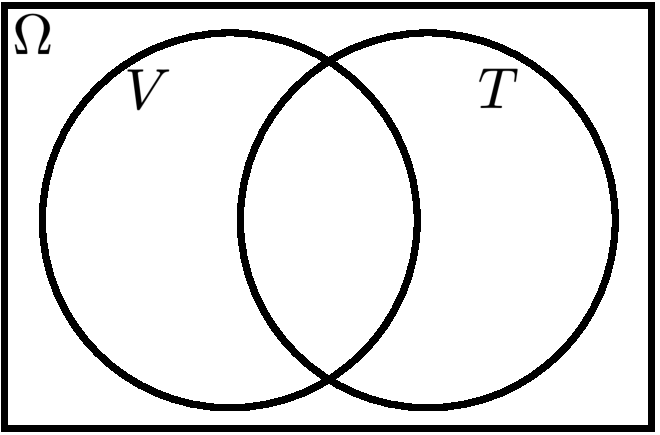
\includegraphics[width = 0.9\linewidth]{./figures/vt}

  \note[item]{Let's build up some intuition by thinking about the dartboard analogy.}
  \note[item]{Event V for volleyball player is an area on the board.}
  \note[item]{If all you know is that the dart hit the board randomly, the probability that it's in V is the area of V divided by the area of the entire sample space (which we assume to be 1).}
  \note[item]{Now what if I tell you that the dart landed somewhere in T, meaning tall?  What does your intuition say?}
  \note[item]{Well, now you don't care about the rest of $\Omega$, right?  You might think let's look inside T and see how much of the area is also inside V. that is exactly what we call conditional probability.}
\end{frame}



\begin{frame}
  \frametitle{Conditional Probability, Part II}
  \begin{block}{Conditional probability}
    For events $A, B \in \Omega$ with $P(B) > 0$, define the \textit{conditional
      probability} of $A$ given $B$ to be
    \[
      P(A|B) = \frac{P(A \cap B)}{P(B)}
      \]
    \end{block}
    \begin{center} 
      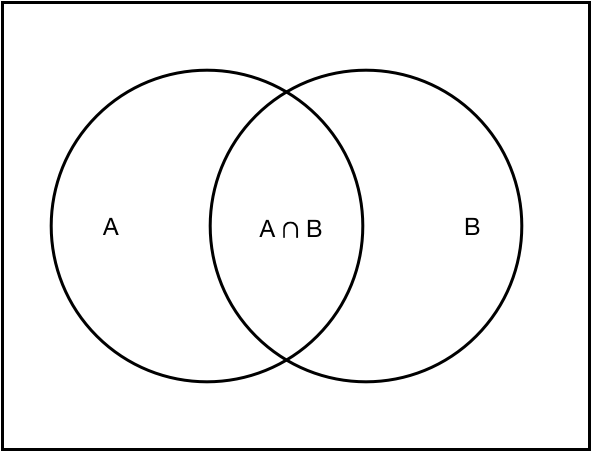
\includegraphics[width = 0.5\linewidth]{./figures/a_and_b}
    \end{center} 
    \note[item]{Here's the formal definition.  the conditional probability of A given B is a ratio.}
    \note[item]{On the top we have the intersection.  on the bottom we have all of B}
\end{frame}

\begin{frame}
  \frametitle{Conditional Probability, Part III}
  \begin{block}{Conditional probability}
    For events $A, B \in \Omega$ with $P(B) > 0$, define the \textit{conditional
      probability} of $A$ given $B$ to be
    \[
      P(A|B) = \frac{P(A \cap B)}{P(B)}
      \]
    \end{block}
    \begin{center} 
      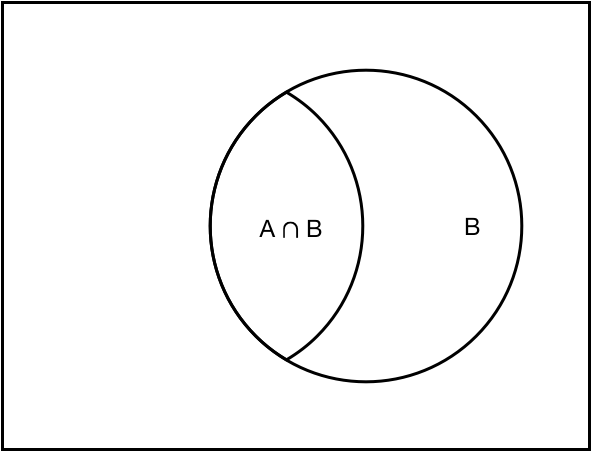
\includegraphics[width = 0.5\linewidth]{./figures/a_given_b}
    \end{center} 
    \note[item]{The idea is we're dropping everything in the sample space outside of B - it's not relevant, and then we have to rescale the probability so everything adds up to 1.}
\end{frame}


\begin{frame}
  \frametitle{Conditional Probability, Part IV}
      \begin{block}{Multiplicative Law of Probability}
      Rearranging the conditional probability statement minimally
      produces the \textit{Multiplicative Law of Probability}.

      For $A, B \in \Omega$ with $P(B) > 0$,

      \[
        P(A|B)P(B) = P(A \cap B) \pause = P(B|A)P(A)
      \]
    \end{block}
    \note[item]{\paul{Suggest deleting the text and just talking through it, this one's pretty simple.}}

\note[item]{This is an important relationship.  It gives us an intuitive way to compute the probability that A AND B occur. }
\note[item]{First, you write down the probability that A occurs.  then, you assume that A has occurred, and you multiply by the probability, which is conditional, that B also occurs.}
\note[item]{\paul{Also suggest handwriting the P(B|A)P(A).  we're going to use that to prove a very famous rule, called Bayes' Rule}}
\end{frame}


\section{Learnosity Check}

\begin{frame}
  \frametitle{}
  Suppose that the probability that a student plays volleyball is .4, the probability that the student is tall is .5, and the probability that the student is both tall and plays volleyball is .3.
  
  What is the conditional probability that the student plays volleyball, given that they are tall?
  
  \paul{Answer: .6}
\end{frame}




\section{Reading: Bayes' Rule}



\begin{frame}
  \frametitle{Reading: Bayes' Rule}
  Read from the top of page 11 to the end of page 13.
\end{frame}



\section{Total Probability}

\begin{frame}
\note[item]{In a lot of probability problems, you need to compute the probability of some complicated event.}
\note[item]{That can be hard to do directly, and you want some way to break down the problem.}
\note[item]{There is a famous technique that helps in a lot of cases.  it's called the law of total probability.}
\note[item]{The idea is we can use a partition of $\Omega$ to break down any event.}
\note[item]{Let's see a picture and then read the law carefully...}
  \frametitle{Total Probability, Part I}
  \begin{block}{The Law of Total Probability}
    If$\ A_{1}, A_{2}, \dots, A_{n}$ is a partition of $\Omega$, and
    if $B \in \Omega$, then
    \[
      P(B) = \sum_{i} P(B \cap A_{i})
    \]
    If there is a positive probability for each partition $A_{i}$,
    then by the \textit{Multiplicative Law of Probability}
    \[
      P(B) = \sum_{i} P(B | A_{i})P(A_{i})
    \]
  \end{block}
\end{frame}

\begin{frame}
  \frametitle{Total Probability, Part II}
  \begin{center}
    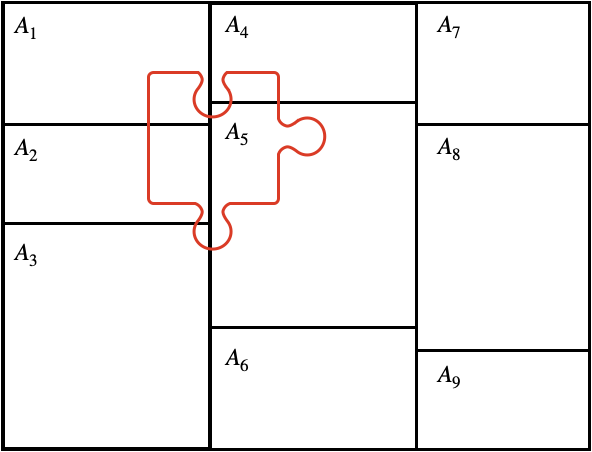
\includegraphics[width=0.75\linewidth]{./figures/total_probability_0}
  \end{center} 
\end{frame}

\begin{frame}
  \frametitle{Total Probability, Part III}
  \begin{center}
    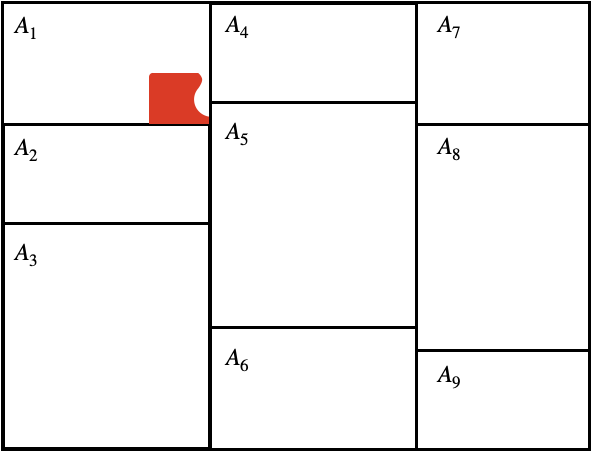
\includegraphics[width=0.75\linewidth]{./figures/total_probability_1}
  \end{center} 
\end{frame}

\begin{frame}
  \frametitle{Total Probability, Part IV}
  \begin{center}
    
\includegraphics[width=0.75\linewidth]{./figures/total_probability_2}
  \end{center} 
\end{frame}

\begin{frame}
  \frametitle{Total Probability, Part V}
  \begin{center}
    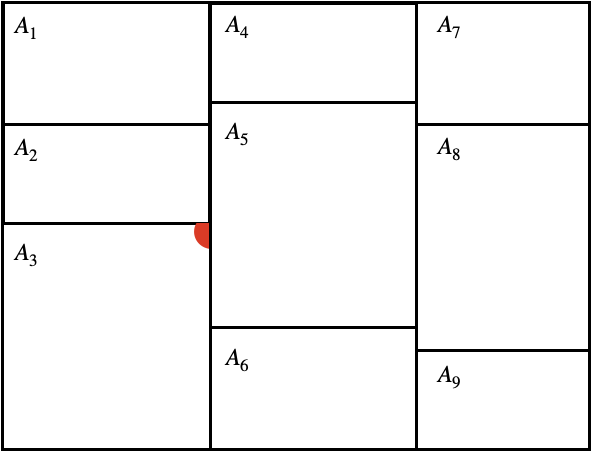
\includegraphics[width=0.75\linewidth]{./figures/total_probability_3}
  \end{center} 
\end{frame}

\begin{frame}
  \frametitle{Total Probability, Part VI}
  \begin{center}
    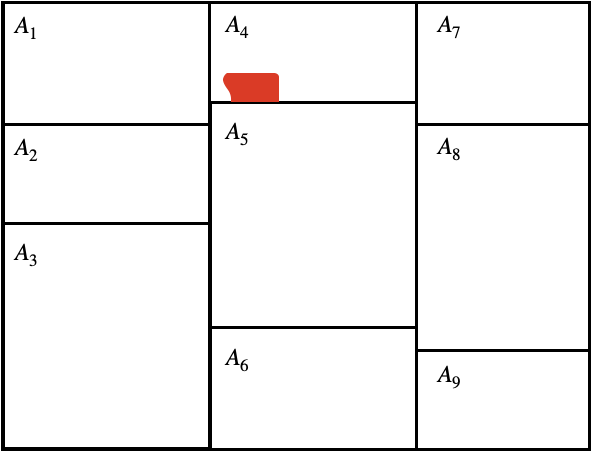
\includegraphics[width=0.75\linewidth]{./figures/total_probability_4}
  \end{center} 
\end{frame}

\begin{frame}
  \frametitle{Total Probability, Part VII}
  \begin{center}
    
\includegraphics[width=0.75\linewidth]{./figures/total_probability_5}
  \end{center} 
\end{frame}

\begin{frame}
  \frametitle{Total Probability, Part VIII}
  \begin{center}
    
\includegraphics[width=0.75\linewidth]{./figures/total_probability_6}
  \end{center} 
\end{frame}


\begin{frame}
\note[item]{Now let's carefully read the law of total probability.}
\note[item]{The probability of B is a sum, if you look inside the sum, what we do is we intersect B with some $A_i$, which is part of the partition, then take the probability.}
\note[item]{To finish the law, we can then apply the multiplication rule.  we write each of these joint probabilities as a product.  First, we take the probability we're inside $A_i$, then multiply it by the conditional probability that we're also in B.}
\note[item]{That's the law of total probability.  It can be quite useful, if you can think of a good partition.}
  \frametitle{Total Probability, Part I}
  \begin{block}{The Law of Total Probability}
    If$\ A_{1}, A_{2}, \dots, A_{n}$ is a partition of $\Omega$, and
    if $B \in \Omega$, then
    \[
      P(B) = \sum_{i} P(B \cap A_{i})
    \]
    If there is a positive probability for each partition $A_{i}$,
    then by the \textit{Multiplicative Law of Probability}
    \[
      P(B) = \sum_{i} P(B | A_{i})P(A_{i})
    \]
  \end{block}
\end{frame}


\section{Bayes' Rule}

\begin{frame}
  \frametitle{Conditional Inverses}
  \note[item]{We know about conditional probability.  Let's say we have two events X and Y.  Are these two conditional probabilities the same?}
  \note[item]{In fact, the answer is usually no.  here's an example to convince you. <read>}
  \note[item]{There is an easy way to get from one of these probabilities to the other.  it's the famous theorem known as Bayes' Rule.}
 \begin{center} Does $P(X|Y) = P(Y|X)$? \end{center}
  
  \pause
  Example: 
\begin{itemize}
\item   $X =$ Visited Berkeley
\item  $Y = $ Attend MIDS
\end{itemize}

\end{frame}


\begin{frame}
  \frametitle{Deriving Bayes' Rule}
  
  \note[item]{Deriving Bayes' Rule is easy.  We start with the probability of X and Y.  Then wewrite the multiplication rule two ways.}
  \note[item]{ $P(Y)P(X|Y)=$.  and $=P(X)P(Y|X)$.}
  \note[item]{Divide: $P(X|Y) = \frac{P(Y|X)P(X)}{P(Y) } $}
 \note[item]{That's Bayes's Rule!  It's easy to derive if you ever forget it.}
  
 \vspace{-2cm} $$P(X \cap Y)$$

\end{frame}


\begin{frame}[t]
  \frametitle{Bayes' Rule Example}
  \note[item]{Why is Baye's rule important?  It can tell us how to adjust probabilities of hypotheses in response to evidence.}
  \note[item]{Let's work through a problem together.  This is a very classic example for Bayes' Rule.}
  
\begin{itemize}
\item A rare disease affects 2 out of 10,000 people.
\item The test is right 99\% of the time for healthy people.
\item The test is right 100\% of the time for sick people.
\end{itemize}


Given that you get a positive test, what is the probability that you have the disease?

\note[item]{You can see that this sounds quite scary, right?  the test is correct 99\% of the time.}

\begin{itemize}
\item Let D be the event you have the disease
\item Let T be the event the test is positive.
\end{itemize}

\note[item]{Write down what we know: $P(D) = .0002$,$ P(D^C) = .9998$, $P(T|D)=1$, $P(T|D^C) = .01$}
\end{frame}



\begin{frame}[t]
  \frametitle{Bayes' Rule Example Cont.}

We know:  $P(D) = .0002,  P(D^C) = .9998$\\
 $\qquad \qquad \ \  P(T|D)=1, P(T|D^C) = .01$


We want: $P(D|T)$

\note[item]{$P(D|T) = \frac{P(T|D)P(D)}{P(T)}$ }
\note[item]{Still missing $P(T)$.  Can use law of total probability, using D for partition.}
\note[item]{$P(T) = P(D)P(T|D) + P(D^C)P(T|D^C)$  }
\note[item]{$P(D|T) = \frac{P(T|D)P(D)}{P(T)} =  \frac{P(T|D)P(D)}{ P(D)P(T|D) + P(D^C)P(T|D^C) = .0196}$}
\note[item]{Even though the test is 99\% accurate, there is still less than a 2\% chance you have the disease.}
\end{frame}


\begin{frame}
  \frametitle{Bayesian Statistics}
  
  \note[item]{Bayes' Rule is the foundation of an entire school of stats.}
  \note[item]{Let me try to compress an entire school into 60 seconds.}
  \note[item]{In bayesian stats, we may be interested in some hypothesis.  Let H be the event that it's true.}
  \note[item]{To a mainstream statistician, that doesn't make any sense, a hypothesis is true or false.}
  \note[item]{To a bayesian, probability is used to represent your personal subjective belief.  before you see the data, you give the hypothesis a prior probability, P(H)}
  \note[item]{Then you see data, D.  you can use bayes rule to update your probability to $P(H|D)$.  this is your posterior.  }
  
  Let H be the event a hypothesis is true.
  \begin{itemize}
\item We begin with prior (subjective) belief $P(H)$
\end{itemize}

  Let D be the data we collect
  \begin{itemize}
\item Use Bayes' Rule to compute posterior belief, $P(H|D)$.
\end{itemize}

\note[item]{There's your 60 second crash course on Bayesian stats.}
\end{frame}





%
%\begin{frame}[t]
%  \frametitle{Bayes' Rule Example 1}
%  \begin{exampleblock}{Shy voters}
%    In the 2016 Presidential election, Nate Silver's 538 predicted a
%    win for Hillary Clinton based off the current polls. Hillary
%    Clinton did not win the election. \textit{What went wrong with the
%      polling?} 
%  \end{exampleblock}
%\end{frame}
%
%\begin{frame}[t]
%  \frametitle{Bayes' Rule Example 1 (cont.)}
%  \begin{exampleblock}{Shy voters}
%    Polls require that people will talk to you. Let $C$ be the event
%    that someone will vote for Clinton, and let the \textit{true}
%    $P(C) = 0.45$.
%    \begin{itemize}
%      \item Because there were only two effective candidates, what is
%        $P(C^{C})$?
%      \end{itemize}
%      Let the event $A$ be that the voter answers a poll when called. 
%    Suppose that Clinton voters were willing to answer a phone poll
%    40\% of the time, $P(A|C) = 0.4$. Suppose that supporters of the
%    other candidate were more bashful; $P(A|C^{C}) = 0.3$.
%
%    \begin{itemize}
%      \item Write out the Probability that you actually calculate when you
%        conduct a poll. \pause
%      \item $P(C | A)$, which is not $P(C)$. 
%      \item Given the problem setup, what do you produce from this
%        calculation? How different is this from $P(C)$? 
%    \end{itemize} 
%  \end{exampleblock}
%\end{frame}
%
%



\section{Reading: Independence}

\begin{frame}
  \frametitle{Reading: Independence}
  Read section 1.1.4, Independence of Events
\end{frame}


\section{Independence}

\begin{frame}
  \frametitle{Independence}

\note[item]{Let's take a look at the formal definition of independence.  Notice that we use the elegant product equation.  This version is a bit more universal.  If event have probability zero, there may not be a good way to define conditional probability. }
  \begin{block}{Independence of events}
    Events $A, B \in S$ are \textit{independent} if $P(A \cap B) =
    P(A)P(B)$. 
  \end{block}

\vspace{1cm}
\pause
\note[item]{However, as long as the events have nonzero probability, you can also write independence in terms of conditional probabilities.}
    \begin{block}{Theorem: conditional probability and independence}
    For $A, B \in S$ and $P(B)>0$, $A$ and $B$ are
    independent if and only if $P(A|B) = P(A)$.
  \end{block}
\end{frame}

\begin{frame}[t]
  \frametitle{Conditional Probability and Information}
  \note[item]{We introduced conditional probability, and we can think about it in terms of information.}
  

    \begin{columns}
\begin{column}{0.65\textwidth}
\begin{itemize}
\item   Let $C$ be event that our subscriber cancels.
  \item Let $W$ be the event our subscriber waited 2 hours on the phone.
\end{itemize}


 $$ P(C) < P(C | W) $$ 
 
 $W$ gives us \textit{information} about C. 
 \end{column}
\begin{column}{0.35\textwidth}  %%<--- here
    \begin{center}
     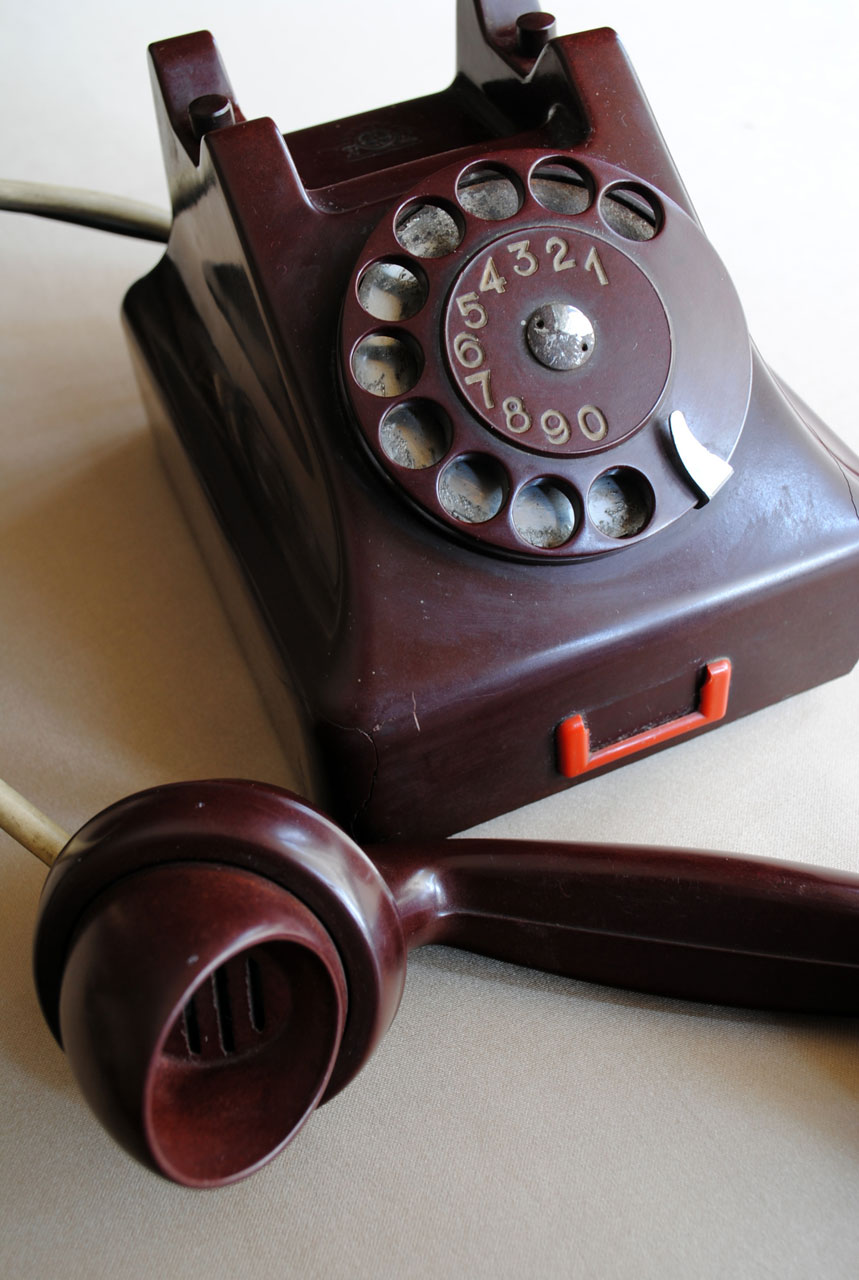
\includegraphics[width=\textwidth]{figures/phone}
     \end{center}
\end{column}
\end{columns}

\note[item]{This is what we usually expect, at least a little bit.  one event will give us some information about another event.  But it's not always the case.}
\end{frame}



\begin{frame}[t]
  \frametitle{Understanding Independence}
  \note[item]{Same situation, but now let H be the event the subscriber hates cilantro.}
  \note[item]{Now, does knowing that the subscriber hates cilantro give us any information about whether they cancel?}
  
  \begin{columns}
\begin{column}{0.65\textwidth}
\begin{itemize}
\item   Let $C$ be event that our subscriber cancels.
  \item Let $H$ be the event our subscriber hates cilantro.
\end{itemize}

   Is $P(C)$ different from $ P(C | H)$?
\end{column}
\begin{column}{0.35\textwidth}  %%<--- here
    \begin{center}
     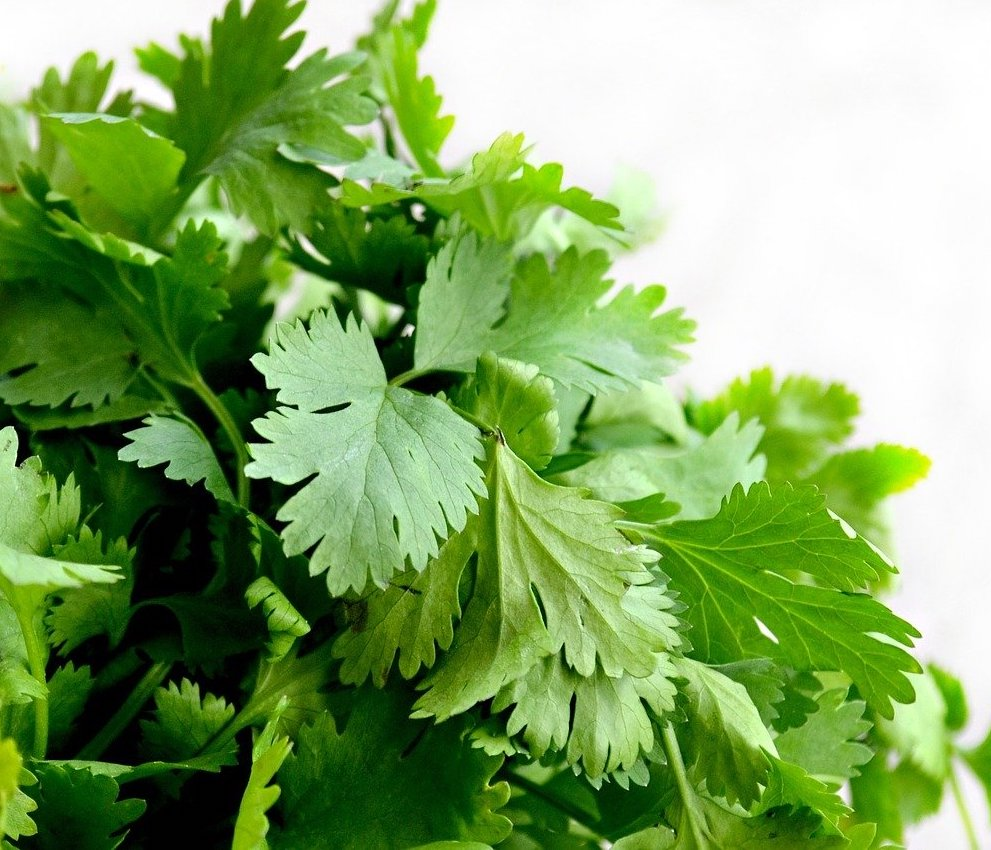
\includegraphics[width=\textwidth]{figures/cilantro}
     \end{center}
\end{column}
\end{columns}
  


 
\note[item]{That's pretty farfetched, right?  Unless you're actually sending cilantro to your subscribers - let's assume that's not the case - these events have nothing to do with each other.  So $ P(C) = P(C|H) $. }
\note[item]{Let's play with the math.  $P(C|H) = P(C \cap H)/P(H)$ }
\note[item]{So $P(C \cap H) = P(C)P(H)$.  This is a really elegant formula.}
\note[item]{Also, $P(H) = P(C \cap H) / P(C) = P(H | C)$.  So if H gives no info about C, C gives no info about H.}
\end{frame}









\begin{frame}
  \frametitle{Importance of Independence}
  \note[item]{My cilantro example is pretty silly.  So why do we need independence?}
  \note[item]{It's going to become very important when we talk about sampling.}

Later in the course: In a \textit{random sample} every unit is independent of every other unit.




  \begin{columns}
\begin{column}{0.65\textwidth}
Survey Example:

\begin{itemize}
\item Let $D_1$ be event that the first respondent has a dog.
\item Let $D_2$ be event that the second respondent has a dog.
\item \dots 
\end{itemize}

\end{column}
\begin{column}{0.35\textwidth}  %%<--- here
    \begin{center}
     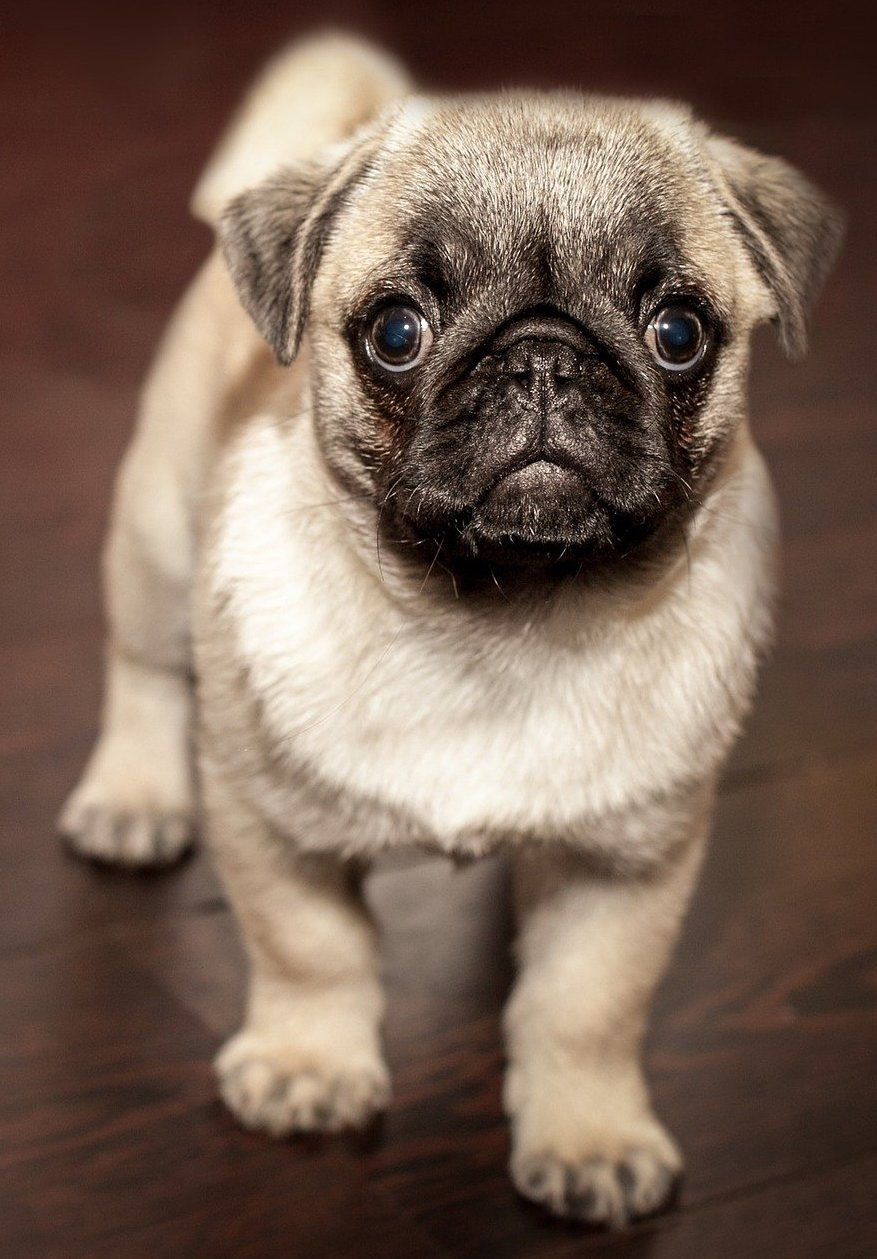
\includegraphics[width=\textwidth]{figures/pug}
     \end{center}
\end{column}
\end{columns}

  \note[item]{Think of a survey. <read>}
  \note[item]{  if $D_1$ and $D_2$ are independent, you learn just as much from the second as you do from the first - that's good!}
  \note[item]{But what it they are family members?  Then the responses of the first one probably does give you information about the second.  This makes it much harder to analyze the data.  Throughout this course, we always want to be skeptical about whether independence holds, but many of our techniques really will require it to work.}

\end{frame}






\section{Framing the Following Segment}

\begin{frame}
  \frametitle{Fatal Officer Involved Shootings}

  We're going to take on an important, but challenging topic here -- the use of police force.

  \begin{itemize}
      \item In particular, we're going to read a paper that investigates whether office race plays any role in disparate use of force against people of color
    \item This is an important, durable question and one that at the time that we're putting the course together is the predominant political issue.
  \end{itemize}
\end{frame} 

\begin{frame}
  \frametitle{Fatal Officer Involved Shootings} 
  As faculty, we stand is solidarity with people of color, without exception and without qualification.

  \begin{itemize}
    \item We're going to read an academic, data-based conversation where the authors come to the conclusion that there is no evidence of differential treatment of people of color by white officers.
    \item And, we're going to critically engage with this article, to assess whether the data supports this claim 
  \end{itemize}
\end{frame}

\section{Probability and Police Shootings}

\begin{frame}[standout]
  Are Black citizens subjected to unfairly violent treatment by law enforcement?
\note[item]{\paul{Instead, I'd lead with just the question on a slide for the punchiest opening. }}
\note[item]{Let's start our discussion of probability with this question... <read>  }
\note[item]{This is a matter that we care deeply about (as I'm sure
  many of our students do), but I want to make clear that we want to
  approach it today from an academic perspective - that means being
  dispassionate and using data to construct measurements that aren't
  biased by our personal convictions.} 
\end{frame}



\begin{frame}
  \frametitle{Johnson et al. (2019) }
    \begin{block}{Johnson et al. (2019)}
    Are minority groups subjected to unfairly violent treatment
    by law enforcement?  
  \begin{enumerate}
  \item Are Black civilians overrepresented in FOIS?
  \item If so, is this because of racial discrimination by White
    officers?
  \end{enumerate}
  \end{block} 

  \note[item]{\paul{This slide also feels out of place.  Why not fully
      describe the question and the difficulty of defining fairness,
      then present the specific paper?}} 
  \note[item]{\paul{Suggest deleting this, and replacing with a
      modified slide after the next one.}}
    \begin{itemize}
  \item Develop Database that is a near-total recording of all \textit{fatal officer
      involved shootings} (FOIS) in the US in 2015.
  \item ``Model'' whether race of civilian is a factor that
    predicts being involved in a FOIS.
  \end{itemize}
  
  % Three outcomes can occur when an officer fires their weapon:
  % \begin{enumerate}
  % \item The payload does not hit the civilian
  % \item The payload does hit the civilian, but does not kill them
  % \item The payload hits the civilian, and kills them
  % \end{enumerate}
\end{frame}

\begin{frame}
  \frametitle{Johnson et al. (2019) Conclusions}
  \begin{block}{Study conclusions}
    \begin{itemize}
    \item \textit{``We find no overall evidence of anti-Black or
        anti-Hispanic disparities in fatal shootings.''}
    \item \textit{``White officers are not more likely to shoot minority
        civilians than non-White officers.''}
    \end{itemize} 
  \end{block}
\end{frame}

\begin{frame}
  \frametitle{Probability Translation} 
  Crystal clear probability statement about officer race:
  \begin{align*}
    P(\text{shot} &| \text{minority civilian, white officer}, X) \leq\\ 
                  & P(\text{shot} | \text{minority civilian, minority officer}, X)
  \end{align*}
  \note[item]{The answer to this probability statement informs policy: If true,
    then take proactive measures in hiring}
  Question: Is it possible to justify this statement using only data of officer shootings?
  
  \note[item]{\paul{Is this the claim you want to attack?  for
      example, they also say "we find no overall evidence of
      anti-Black or antiHispanic disparities in fatal shootings".  and
      "Thus, in the typical shooting, we did not find evidence 
      of anti-Black or anti-Hispanic disparity." which seems absurd
      and more directed at the research question.}} 
  \note[item]{\paul{Is the problem that in the two quotes above,
      "racial disparity" is not properly defined?   but the statement
      about office race is precise enough to be clearly attacked?  If
      that's your thinking, I can get behind this strategy. probably
      need to end the modeling (claims to) save the day slide with the
      bullet about "if the officer's whiteness is predicitive..."  }} 
\end{frame}

\begin{frame}
  \frametitle{Measuring Fairness}
  \begin{itemize}
  \item Twenty-six percent of civilians killed by police shootings in 2015 were
    Black.
  \item The U.S. population is 12\% Black.
  \end{itemize}
  \note[item]{\textbf{We need these numbers} 
    - Rates of interactions between black civilians and police are different
    - Rates of violent crimes committed by black and white civilians.} 
  \note[item]{We could control for interactions with police. But,
    there are all kinds of reasons that these interactions -- set by
    policy -- are different between groups. The Oakland police are
    under federal receivership because of their treatment.} 
  \begin{itemize}
  \item White and Black civilians have different rates of exposure
    to situations that might result in FOIS.
  \end{itemize}
\end{frame}

\end{document}
